\documentclass[paper=a4, twoside=true, fontsize=11pt, ]{scrbook}

%%%----------------------------------------------------------------
%%% ENCODING AND FONTS
\usepackage[utf8]{inputenc} % input encoding
\usepackage{times}          % general
\usepackage{helvet}         % sans serif
\usepackage[T1]{fontenc}    % font encoding

%% special symbols
\usepackage{pifont}% http://ctan.org/pkg/pifont
\newcommand{\cmark}{\ding{51}}%
\newcommand{\xmark}{\ding{55}}%

%%%----------------------------------------------------------------
%%% DOCUMENT INFO
%% additional variables
\makeatletter
\newcommand\reporttype[1]{\def\@reporttype{#1}}
\newcommand\timespan[1]{\def\@timespan{#1}}
\newcommand\group[1]{\def\@group{#1}}
\newcommand\supervisor[1]{\def\@supervisor{#1}}
\newcommand\chiefsupervisor[1]{\def\@chiefsupervisor{#1}}
\makeatother

%% entries
\title{Failure behavior of unidirectional Carbon Fiber-Reinforced Composite (CFRP)}
\subtitle{Experimental investigation and comparison with an existing failure criterion}
\reporttype{Semester Thesis}
\author{Roman Rüttimann}
\supervisor{Arthur Girard}
\chiefsupervisor{Prof. Dr. Dirk Mohr}
\group{Chair of Computational Modeling of Materials in Manufacturing}
\timespan{Autumn Semester 2019}
\date{\today}

%%%----------------------------------------------------------------
%%% PATHS
\newcommand*{\texpath}{content}
\newcommand*{\imgpath}{img}

%%%----------------------------------------------------------------
%%% INITIALIZE
%%%----------------------------------------------------------------
%%% COLORS
\usepackage{xcolor}       % color commands

%%%----------------------------------------------------------------
%%% MATH
\usepackage{amsmath}      % principal math package
\usepackage{amssymb}      % extended math symbols
\usepackage{amsthm}       % improved theorem definition
\usepackage{physics}      % simplified commands for physics notation
\usepackage{siunitx}      % consistent SI-units
  \sisetup{per-mode=symbol-or-fraction,range-phrase=\dots,range-units=single}

%%%----------------------------------------------------------------
%%% LISTS
\usepackage{enumitem}

%%%----------------------------------------------------------------
%%% FIGURES
\usepackage{float}        % floating figures (do not use in KOMA script)
\usepackage{scrhack}      % fixes floating environments in KOMA script 
\usepackage[pdftex]{graphicx}   % improved includegraphics
\usepackage{rotating}     % rotate graphics (load after graphicx)

%%%----------------------------------------------------------------
%%% TABLES
\usepackage{booktabs}     % better spacing
\usepackage{longtable}    % multi page tables
\usepackage{colortbl}     % allows to color cell backgrounds

%%%----------------------------------------------------------------
%%% LABELS
\usepackage{showkeys}     % DEBUGGING show labels abover references

% %%%----------------------------------------------------------------
% %%% CAPTIONS
\usepackage[
  font={small,sl},        % small, italic
  hang,                   % hanging
  labelfont=bf            % bold label
  ]{caption}              % captions for tables and figures
%\usepackage{captcont}     % subfigures over multiple pages

%%%----------------------------------------------------------------
%%% PAGE STYLE
\usepackage{scrlayer-scrpage}   % enhanced header editing in KOMA-Script
\KOMAoptions{
  DIV=8,                   % type area, the larger the factor, the larger the text block
  BCOR=10mm,                % binding correction
  headinclude=true,         % insert header space
  headings=twolinechapter,  % chapter in two lines
  numbers=noenddot          % all numbers of setioning commands are set without a final point
}
\usepackage{microtype}      % better text spacing

\topmargin  -12.7mm
\textheight 234.0mm
\textwidth  160.0mm
\oddsidemargin   4.57mm
\evensidemargin -5.59mm
\parskip   2.54mm
\parindent 0mm
\headsep  15mm
%\footskip 10mm

\renewcommand{\arraystretch}{1.5}
\renewcommand{\baselinestretch}{1}

%%----------------------------------------------------------------
%% BIBLIOGRAPHY
\usepackage[backend=biber,style=numeric-verb,url=false,doi=false,isbn=false]{biblatex}

%%%----------------------------------------------------------------
%%% REFERENCING
\makeatletter
\usepackage[
  pdftex,                       % pdftex backend
  bookmarks,                    % make bookmarks
  bookmarksopen=true,           % open bookmarks tree
  bookmarksnumbered=true,       % put section numbers in bookmarks
  pdfauthor={\@author},         % text for pdf author name
  pdftitle=\@title: \@subtitle, % text for pdf title name
  colorlinks=false,             % box hyperlinks
  linkcolor=black,              % textcolor of links
  citecolor=black,              % textcolor of citation links
  filecolor=black,              % textcolor of file links
  urlcolor=black,               % textcolor of url links
  anchorcolor=black,            % anchor color
  menucolor=black,              % color of menu links
  breaklinks=true,              % allow links to break over multiple lines
  pageanchor=true,              % for jumping to a page
  plainpages=false,             % page number anchors as plain arabic
  pdfpagelabels=true]{hyperref}
\makeatother

%%----------------------------------------------------------------
%% TOOLKITS
\usepackage{csquotes}     % Advanced quotation tools
\usepackage{pdfpages}     % include full pdf pages
\usepackage{tcolorbox}    % colored text boxes
  \tcbuselibrary{skins}
\usepackage{currfile}     % get path information about current file
\usepackage{tikz}

\begin{comment}
%%%----------------------------------------------------------------
%%% BIBLIOGRAPHY URL LINKS
% format that applies a hypertext reference
\DeclareFieldFormat{linked}{%
  \ifboolexpr{ test {\ifhyperref} and not test {\ifentrytype{online}} }
    {\iffieldundef{doi}
       {\iffieldundef{url}
          {\iffieldundef{isbn}
             {\iffieldundef{issn}
                {#1}
                {\href{https://portal.issn.org/resource/ISSN/\thefield{issn}}{#1}}}
             {\href{https://books.google.com/books?vid=ISBN\thefield{isbn}}{#1}}}
          {\href{\thefield{url}}{#1}}}
       {\href{http://dx.doi.org/\thefield{doi}}{#1}}}
    {#1}}

% Define new command that returns the first word of a given field
\makeatletter
\def\thefieldfirstword#1{%
  \expandafter\expandafter
  \expandafter\firstword
  \expandafter\expandafter
  \expandafter{\csname abx@field@#1\endcsname}}
\def\firstword#1{\firstword@i#1 \@nil}
\def\firstword@i#1 #2\@nil{#1}
\makeatother

% Redefine url format to print only first URL, omit URL prefix
\DeclareFieldFormat{url}{\url{\firstword{#1}}}

\renewbibmacro*{title}{% Based on generic definition from biblatex.def
  \ifboolexpr{ test {\iffieldundef{title}} and test {\iffieldundef{subtitle}} }
    {}
    {\printtext[title]{\printtext[linked]{%
       \printfield[titlecase]{title}%
       \setunit{\subtitlepunct}%
       \printfield[titlecase]{subtitle}}}%
     \newunit}%
  \printfield{titleaddon}}

\renewbibmacro*{periodical}{% Based on generic definition from biblatex.def
  \iffieldundef{title}
    {}
    {\printtext[title]{\printtext[linked]{%
       \printfield[titlecase]{title}%
       \setunit{\subtitlepunct}%
       \printfield[titlecase]{subtitle}}}}}

% Don't link titles in citations
\AtEveryCite{\DeclareFieldAlias{linked}{default}}
\end{comment}
\pdfcompresslevel=9
\pdfoutput=1
\DeclareGraphicsExtensions{.pdf,.png}

%%%----------------------------------------------------------------
%%% HEADERS
%\definecolor{laccentcolor}{HTML}{d3d3d3}

\addtokomafont{disposition}{\sffamily}
\addtokomafont{chapter}{\LARGE}

\newif\ifappendix

\def\chaplengths{{11mm,6mm,7mm,2.5mm,7mm,5mm,6mm,7mm,6.5mm}}
\def\applengths{{4mm,8.5mm,6mm}}
\renewcommand*{\chapterformat}{%
  \hfill\begin{tikzpicture}
    \pgfmathsetmacro{\mylength}{\ifappendix\applengths[\arabic{chapter}-1]\else\chaplengths[\arabic{chapter}-1]\fi}
    \node(n)[inner sep=0, outer sep=0,
        font=\fontsize{6cm}{6cm}\selectfont%,text=laccentcolor
      ]{\rule{0pt}{\ht\strutbox}\thechapter};
    \pgfresetboundingbox
    \useasboundingbox(n.south west)rectangle([xshift=-\mylength]n.north east);% bounding box with a fixed height
\end{tikzpicture}%
}

%%%----------------------------------------------------------------
%%% TITLE PAGE
\makeatletter
\renewcommand\maketitle{%
    \pagestyle{empty}
    \begin{center}
    \includegraphics*[width=0.38\textwidth]{\imgpath/title/eth_logo_lang_pos} \hfill
    \vspace{2cm}
    \newline
	\Huge
	\textbf{\textsf{\@title}}\\[0.7cm]
	\Large\@subtitle\\[2.0cm]
	%\includegraphics*[width=0.4\textwidth]{\imgpath/title/mytitlefigure} 
	\vspace{1cm}
	\sffamily\Large
    \@author\\[0.7cm]
	\large\@reporttype\\[0.7cm]
	\begin{tabular}[t]{rl}
	    supervisor: & \@supervisor\\
	    chief supervisor: & \@chiefsupervisor
	\end{tabular}\\[0.7cm]
	\@group
	\end{center}
}
\makeatother

% %% CHAPTER (with numbering)
% \titleformat{\chapter}[block]
%     {\normalfont\Large\bfseries}    % format applied to label+text
%     {}                              % label
%     {1pc}                           % horizontal separation between label and title body
%     {%
%         \noindent\parbox[][4cm][t]{\textwidth - 4\fboxsep}{%
%             \begin{flushright}
%                 \begin{tcolorbox}[
%                     standard jigsaw,
%                     flushright upper,
%                     boxrule=0pt,
%                     frame hidden,
%                     opacityback=0,
%                     width=2.8cm]
%                     \resizebox{1.8cm}{!}{\color{black}\thechapter}%
%                 \end{tcolorbox}
%             \end{flushright}
%         }\\\Huge
%     }                               % before the title body
%     []                              % after the title body

% %% CHAPTER (without numbering)
% \titleformat{name=\chapter,numberless}
%     {\normalfont\Large\bfseries}   % format applied to label+text
%     {\hspace{-1em}}                % label, fix for horizontal spacing
%     {1pc}                          % horizontal separation between label and title body
%     {%
%         \noindent\parbox[][4cm][t]{\textwidth - 4\fboxsep}{%
%         }\\\Huge
%     }                              % before the title body
%     []                             % after the title body

% \addtokomafont{paragraph}{\sffamily}

% \def\mychpstyleintl{%
% {\noindent\setlength{\tabcolsep}{0pt}\setlength{\arrayrulewidth}{2pt}%
% \begin{tabular}{c}
% \\[100pt]
% \begin{tabular}{lr}
% \begin{tabular}{p{0.6\linewidth}}
% \\
% \end{tabular}
% &
% \begin{tabular}{p{0.4\linewidth}}
% \rightline{{%
% \sffamily%
% \fontseries{bx}%
% \fontshape{n}%
% \fontsize{100}{120}%choose baselineskip to be 1.2 times font size
% \selectfont
% \thechapter}}
% \end{tabular}
% \end{tabular}\\[300pt]
% \end{tabular}
% }}
                       % loads all usepackages and changes layout
\addbibresource{references.bib}     % loads bibliography
\newlength{\distTextWidth}          % effective textwidth
\newlength{\distColSep}             % separation gap when using multiple columns
\setlength{\distTextWidth}{\dimexpr\textwidth-\columnsep\relax}
\setlength{\distColSep}{6pt}

%%%----------------------------------------------------------------
%%% DEBUGGING
\usepackage{showkeys}       % DEBUGGING show labels abover references
\usepackage{comment}        % DEBUGGING comment out code with comment environment
\usepackage{lipsum}         % DEBUGGING blind text
\newcommand{\todo}[1]{\textcolor{red}{TODO: #1}\PackageWarning{TODO:}{#1!}} % DEBUGGING todo note

\begin{document}

%%%----------------------------------------------------------------
%%% TITLE PAGE
\maketitle
\cleardoublepage

%%%----------------------------------------------------------------
%%% PREFACE
\frontmatter
\chapter*{Abstract}

For more than half a century the application of reinforced carbon fibre polymers has been pushing the design of lightweight structures to new limits. A number of macroscopic failure criteria evolved that fit the failure prediction of every stress state in unidirectional carbon fibres based on characteristic values in its principal stress states. Despite the abundance of failure criteria the available experimental data to evaluate them is scarce.
\cleardoublepage
%\includepdf{\texpath/plagiat.pdf}
%\cleardoublepage
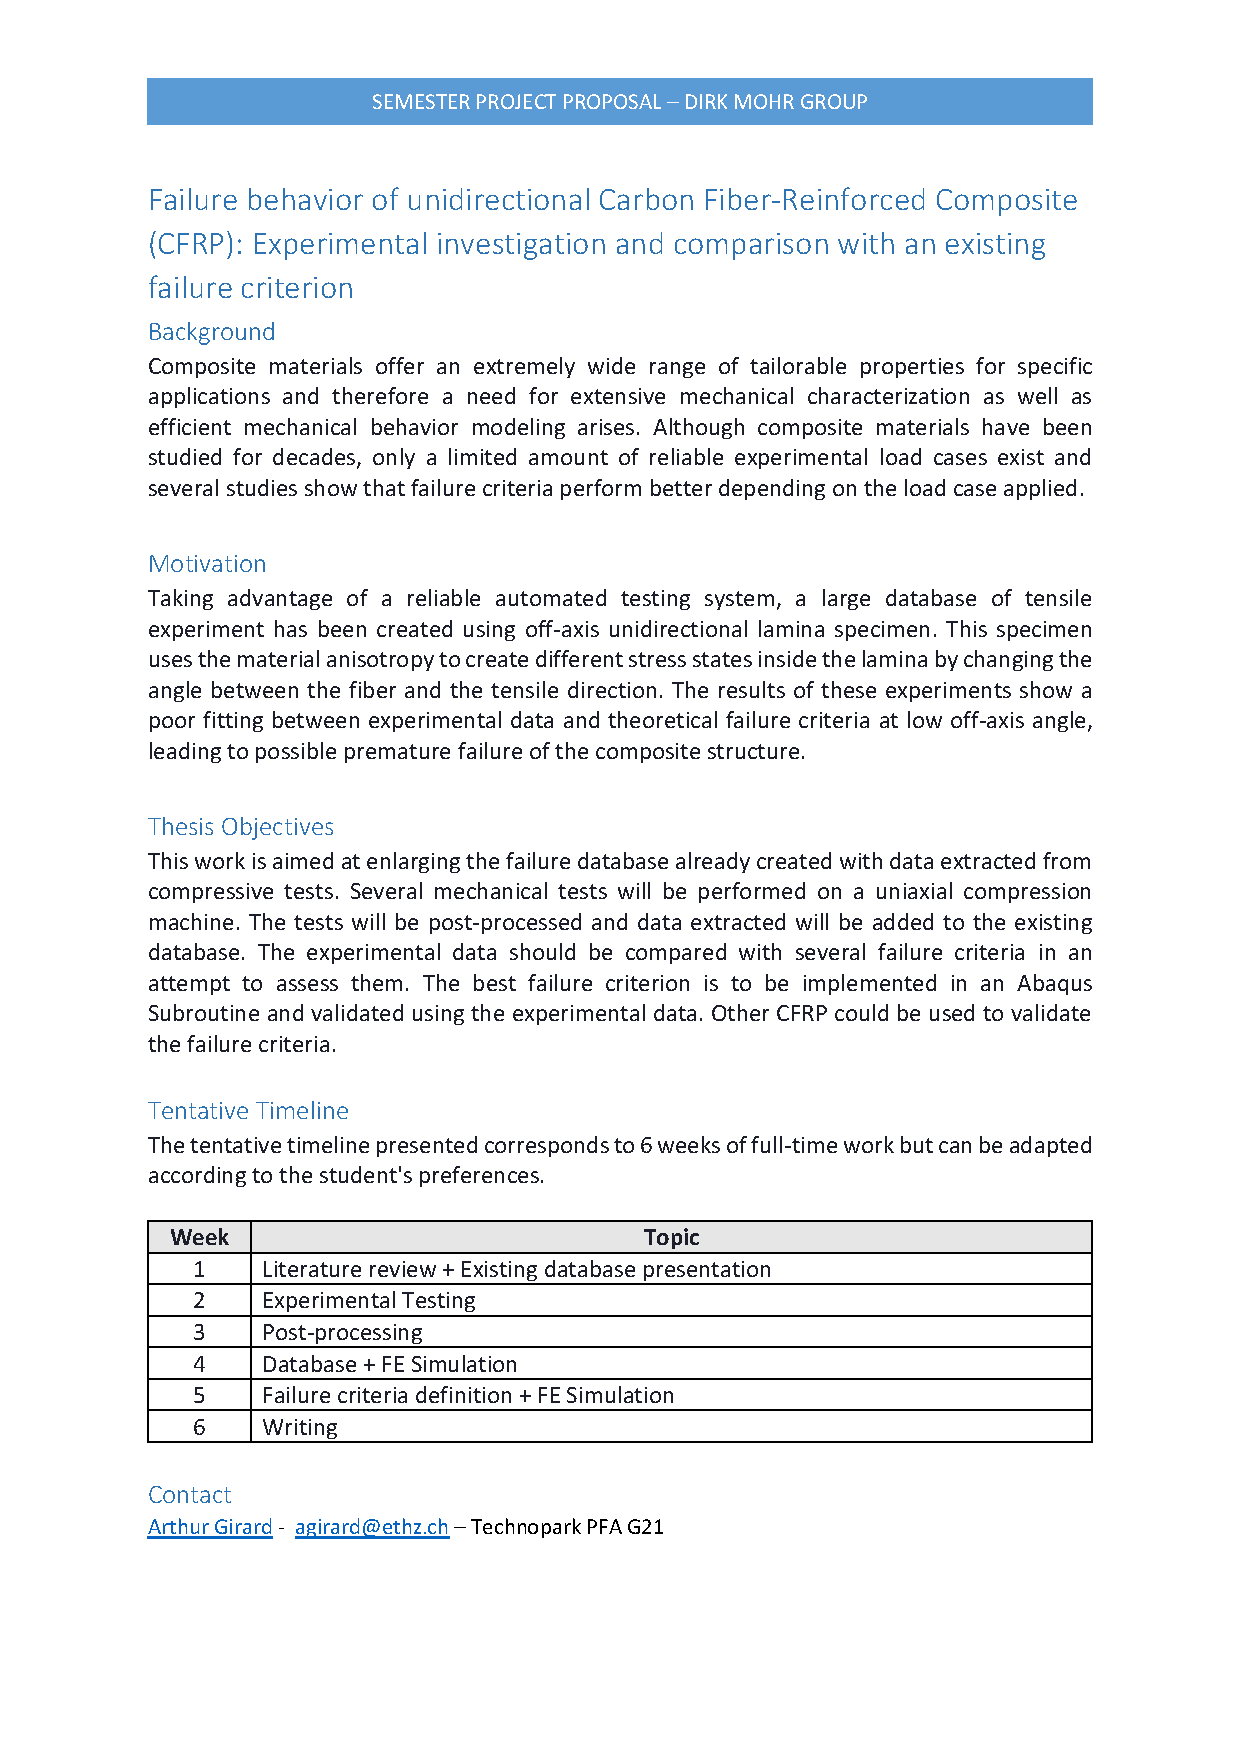
\includepdf{\texpath/task_description.pdf}
\cleardoublepage
\tableofcontents
\cleardoublepage
%\chapter*{List of Symbols}
\label{chap:\currfilebase}

{%
    \renewcommand*{\arraystretch}{1.37}
    \begin{longtable}{@{}l @{\hspace{5mm}} p{0.85\linewidth}}
        CCD     & Charged Coupled Device\\
        PC      & Personal Computer\\
    \end{longtable}
}
\chapter*{List of Abbreviations}
\label{chap:\currfilebase}

{%
    \renewcommand*{\arraystretch}{1.37}
    \begin{longtable}{@{}l @{\hspace{5mm}} p{0.85\linewidth}}
        CCD     & Charged Coupled Device\\
        CLC     & Combined Loading Compression (CLC)\\
        PC      & Personal Computer\\
    \end{longtable}
}
\cleardoublepage

%%%----------------------------------------------------------------
%%% MAIN CONTENT
\mainmatter

\chapter{Introduction}
\label{chap:\currfilebase}

\section{Motivation}
\label{sec:motivation}

\section{Outline}
\label{sec:outline}

\section{State of the Art}
\label{sec:state_of_art}

% The demand for increasing geometric accuracy of precision 5-axis machine tools has reduced the allowed error motions to the extent that error reduction does not suffice while maintaining the productivity and repeatability in a production facility environment. A number of error compensation methods established themselves when it commes to dynamic error motions. Although one of the main reasons causing inaccuracy of machine tools are thermal error motions~{\cite{mayr2012thermal}} the tools used to compensate them specifically are few and far between.\par

% %-----------------------------------------------------
% \section{Target}
% The target of this thesis is to define and carry out measurement tests that allow the characterization of thermally induced error motions on a linear axis of a 5-axis machine tool. The results derived of these tests shall be analysed for a correlation between the temperatures and the deviations measured as well as implemented in a phenomenological model that acts as a non-physical input-output model.

% %-----------------------------------------------------
% \section{Outline}
% First previous studies and the field of research are introduced in the state of the art. Followed by identifying different measurement set-ups and measurement procedures to characterize the thermal error motions occurring along a linear axis in Chapter~{\ref{chap:measurements}}. The evaluation software used to filter and plot the data gathered during the measurement tests is described in the next chapter and the illustration and discussion of the measurement results may be found in Chapter~{\ref{chap:measurementresults}}.  Furthermore a first order model is proposed in Chapter~{\ref{chap:phenomenologicalmodel}}, which represents an area of application the measurement results may be used in future needs. Lastly, a final look on the main difficulties during this thesis and the utility of its results are written down in Chapter~{\ref{chap:conclusionandoutlook}}.

% %-----------------------------------------------------
% \chapter{State of the Art}

% The discussion by Mayr~{\cite{mayr2012thermal}} provides a brief overview of thermal errors in MTs and the known tools to reduce them. This thesis will address thermal geometric errors of a linear axis~{\cite{iso230_3_eng2007}}, their measurement~{\cite{iso230_1_eng2012,iso10791_10_eng2007,iso13041_8_eng2004}} and derived from prior, the modelling of the thermally induced geometric error of the tool center point to the workpiece. Considering the investigations of a similar issue on rotational axes on the very same 5-axis machine tool~{\cite{gebhardt2014high}}, we're given a solid foundation that can be implemented to that task.\par
% The test algorithms are based on a defined standard test~{\cite{iso230_2_eng2014}}. An overview of measurement methods for geometric error motions is provided by Schwenke~{\cite{schwenke2008geometric}} and measurement set-ups espacially suited for 5-axis machine tools are listed by Ibaraki~{\cite{ibaraki2013indirect}}. The utility of a phenomenological model in this area of reasearch is described by Blaser~{\cite{blaser2017adaptive}}.
% In addition the temperature distribution of a three axis milling machine tool was analysed by Huang~{\cite{huang2015real}} and the way of implementing a thermal compensation model to a CNC is described by Liu~{\cite{liu2017robust}}.

% \section{Thermal Sources}
% A multitude of heat sources can cause thermal error motions~{\cite{blaser2017adaptive}}. Considering one linear axis, the main heat sources reduce to environmental temperature change and the heat induced by moving components of the regarded axis. Shi~{\cite{shi2015investigation}} approaches this by modelling a ball screw feed drive expansion in a simplified thermo-mechanical system. In this system the heat is induced through the power loss of the electric motor, the friction between the balls and the races of the two bearings and the friction between the balls and the grooves of the nut (Figure~{\ref{fig:shiballscrewheat}}). Additionally heat convection with the room temperature and the emissivity of all components of the model except the ball screw are neglected due to their significantly smaller surface.

% \begin{figure}[!ht]
% \centering
% \includegraphics[width=0.6\linewidth]{figures/introduction/shiballscrewheat}
% \caption{Thermal consideration of a ball screw drive~{
% \cite{shi2015investigation}}}
% \label{fig:shiballscrewheat}
% \end{figure}

% Note that apart of the heat sources mentioned, the coolant fluid adds an important factor to the thermal behaviour of the machine tool.

% \subsection*{Temperature Gradients}
% MTs are affected by thermal gradients in a variety of ways. Thermal gradients can namely lead to thermal motion errors and occur because of heat sources that exist within the boundaries of the environment. Their existens implies that different parts of the environment have different mean temperatures~{\cite{iso230_3_eng2007}}. But the temperature is not a function of location only. The work of Zhang~{\cite{zhang2017thermal}} shows the periodical fluctuations of the time-varying environmental temperature. And furthermore the investigations conducted by Mayr~{\cite{mayr2015simulation}} concluded in a relation between the environmental temperature change frequency and the TCP displacements occurring on a MT 
% (Figure~{\ref{fig:mayrtemperaturebode}}).

% \begin{figure}[!ht]
% \centering
% \includegraphics[width=0.8\linewidth]{figures/introduction/mayrtemperaturebode}
% \caption{Bode plot of TCP displacements at a measurement position (P1) on the considered X-axis for different environmental change frequencies with an amplitude of {\SI{1}{\kelvin}}. {\SI{100}{\percent}} is the maximum amplitude at axis position P1, $-\SI{210}{\mm}$~{\cite{mayr2015simulation}}}
% \label{fig:mayrtemperaturebode}
% \end{figure}

% \section{Error Motions of Linear Axes}
% The three unwanted transitional movements of a moving component, called linear error motions of a linear axis, are separated into one linear positioning error motion along the direction of motion and two straightness error motions perpendicular to the regarded axis.\par
% The three unwanted rotational movements of a moving component, called angular error motions of a linear axis, are defined as rotations around the three orthogonal axes. They can be separated into one roll motion (around the direction of motion) and two tilts. Note that if the considered axis is horizontal, the tilt around the vertical direction can be called yaw and the tilt around the horizontal direction perpendicular to the direction of motion can be called pitch. The positive sign of the angular error follows the right-hand rule. 

% %!!!(preferably y-axis)
% \begin{figure}[!ht]
% \centering
% \includegraphics[width=0.6\linewidth]{figures/introduction/errorMotions}
% \caption{Error motions of linear axes~{\cite{iso230_1_eng2012}}}
% \label{fig:errorMotions}
% \end{figure}

% where
% \begin{table}[!ht]
% \centering
% \begin{tabular*}{0.9\linewidth}{l p{0.75\linewidth}}
%   \textbf{Symbol} & \textbf{Description} \\ 
%   \midrule
%   $1$				& X-axis commanded linear motion \\
%   $\mathrm{EAX}$	& angular error motion around A-axis (roll) \\
%   $\mathrm{EBX}$	& angular error motion around B-Axis (yaw) \\
%   $\mathrm{ECX}$	& angular error motion around C-axis (pitch) \\
%   $\mathrm{EXX}$	& linear positioning error motion of X-axis; positioning deviations of X-axis \\
%   $\mathrm{EYX}$	& straightness error motion in Y-axis direction \\
%   $\mathrm{EZX}$	& straightness error motion in Z-axis direction \\
% \end{tabular*}
% \caption{Legend to Figure~{\ref{fig:errorMotions}}}
% \label{tab:errorMotions}
% \end{table}
% %!!!
% \section{Measurement of straightness error motions}

% \subsection*{Straightedge and linear displacement sensor}
% In this comparative measurement method a straightedge is used as reference for straightness. A displacement sensor mounted close to the functional point of the moving component allows the measurement of straightness deviations in horizontal or vertical direction depending on the setup of the straightedge.\par
% Unknown errors of the straightedge can be determined and removed from the straightness error motion measurement using the straightedge reversal method. This method applies in the horizontal plane only because of deflection due to gravity in a vertical setup.

% \begin{figure}[!ht]
% \centering
% \subfigure[Normal setup]{
%   \includegraphics[width=0.4\linewidth]{figures/introduction/straightedgenormal}
%   \label{fig:straightedgenormal}
% }\hspace{0.08\linewidth}
% \subfigure[Reversed setup]{
%   \includegraphics[width=0.36\linewidth]{figures/introduction/straightedgereversed}
%   \label{fig:straightedgereversed}
% }
% \caption{Straightedge and linear displacement sensor~{\cite{iso230_1_eng2012}}}
% \label{fig:straightedge}
% \end{figure}

% \begin{table}[!ht]
% \centering
% \begin{tabular*}{0.5\linewidth}{l p{0.4\linewidth}}
%   \textbf{Key} &\\ 
%   \midrule
%   $1$	& straightedge \\
%   $2$	& measurement line \\
%   $3$	& straighedge support points (3) both sides \\
%   $4$	& linear displacement sensor \\
%   $5$	& machine table \\
% \end{tabular*}
% \caption{Legend to Figure~{\ref{fig:straightedge}}}
% \label{tab:straightedge}
% \end{table}

% \subsection*{Microscope and taut wire}
% As straightness reference a steel wire with a diameter near to \SI{0.1}{\mm} is stretched to be approximately parallel to the direction of motion to be checked. The straightness errors are measured using a microscope, or other displacement sensors capable of registering the taut wire deviation perpendicular to the direction of motion. The sensor shall be mounted close to the functional point of the moving component (see Figure~{\ref{fig:microscopetaut}}). The straightness error motion results out of the deviation between taut wire and sensor.\par
% It is not recommended to measure straightness error motions in a vertical plane using this method because it is difficult to determine the sag at any given point.

% \begin{figure}[!ht]
% \centering
% \includegraphics[width=0.35\linewidth]{figures/introduction/microscopetaut}
% \caption{Staightness error measurement using taut wire and microscope~{\cite{iso230_1_eng2012}}}
% \label{fig:microscopetaut}
% \end{figure}

% \begin{table}[!ht]
% \centering
% \begin{tabular*}{0.3\linewidth}{l p{0.2\linewidth}}
%   \textbf{Key} &\\ 
%   \midrule
%   $1$	& spindle \\
%   $2$	& microscope \\
%   $3$	& taut wire \\
%   $4$	& weight \\
%   $5$	& table \\
% \end{tabular*}
% \caption{Legend to Figure~{\ref{fig:microscopetaut}}}
% \label{tab:microscopetaut}
% \end{table}

% \subsection*{Alignment telescope}
% When using an alignment telescope the telescope shall be mounted on the table and the target shall be mounted on the tool holder. The optical axis of the telescope serves as straightness reference (see Figure~{\ref{fig:alignmenttelescope}}).\par
% Local bending causes the optical line of the telescope to change position. Therefore one should take care in the fixing of the telescope, particularly in situations where bending is suspected.

% \begin{figure}[!ht]
% \centering
% \includegraphics[width=0.6\linewidth]{figures/introduction/alignmenttelescope}
% \caption{Straightness error measurement using alignment telescope~{\cite{iso230_1_eng2012}}}
% \label{fig:alignmenttelescope}
% \end{figure}

% \begin{table}[!ht]
% \centering
% \subtable{%
%   \centering
%   \begin{tabular*}{0.32\linewidth}{l p{0.22\linewidth}}
%     \textbf{Key} &\\ 
%     \midrule
%     $1$	& workpiece side (table) \\
%     $2$	& tool side (position 1) \\
%     $3$	& tool side (position 2) \\
%     $4$	& telescope \\
%     $5$	& reading micrometer \\
%   \end{tabular*}
% }\hspace{0.08\linewidth}
% \subtable{%
%   \centering
%   \begin{tabular*}{0.32\linewidth}{l p{0.22\linewidth}}
%     \textbf{Key} &\\ 
%     \midrule
%     $6$	& reticule \\
%     $7$	& target \\
%     $8$	& light source \\
%     $9$	& measured deviation \\
%   \end{tabular*}
% }%
% \caption{Legend to Figure~{\ref{fig:alignmenttelescope}}}
% \label{tab:alignmenttelescope}
% \end{table}

% \subsection*{Alignment laser}
% Similarly to the alignment telescope the laser head shall be mounted on the component that carries the workpiece and the four-quadrant photo-diode target shall be mounted on the tool carrying side.\par
% The problem of local bending can best be stemmed by fixing the alignment laser on a support simulating a rigid workpiece connected to the table.

% \subsection*{Laser straightness interferometer}
% To measure the relative straightness error motion between the tool and the workpiece, the bi-mirror reflector shall be mounted on the component that carries the workpiece and the Wollaston prism shall be mounted on the component that carries the tool. Optical components and measuring methods differ and should be applied following the manufacturers' instructions.\par
% Local bending causes the centreline of the reflector to change its position. This situation can be rectified by supporting the reflector mounting kinematically.

% %!!! figure?!

% \section{Measurement of linear positioning error motions}

% \subsection*{Laser interferometer\label{sec:laserinterf}}
% The retroreflector mounted on the component that carries the tool and the interferometer mounted on the table allow to measure the relative positioning error motion between the tool and the workpiece. The laser beam emitted from a leaser head shall be parallel to the linear motion as much as possible as misaligning causes cosine error. To compensate for air refraction air sensors, measuring air temperature, pressure and humidity, shall be located near to the beam path.

% %!!! figure?!

% \subsection*{Linear encoder}
% To measure the position between workpiece and tool a scale and a reader shall be mounted on the workpiece and the tool carrying component respectively. The scale shall be mounted as parallel as possible to the measured axis of motion as misalignment causes cosine error.\par
% It is possible to measure one straightness error motion simultaneously when a grid is used as scale.

% %!!! figure?!
% \subsection*{Calibrated ball array}
% The positions of the precision spheres of the ball array artefact (see Figure~{\ref{fig:ballarar}}) in the machine coordinate system are determined by a displacement measuring or a surface detection system. The calibration documentation typically includes the center position of the individual spheres, the sphere size and form measurement uncertainty and the artefact coefficient of thermal expansion. The calibrated center points are normally not exactly equally spaced and thus the position of the target points prescribed in Section~{\ref{sec:meastestalgo}} is partially fulfilled.

% \begin{figure}[!ht]
% \centering
% \subfigure[1D ball array]{
%   \includegraphics[width=0.22\linewidth]{figures/introduction/ballarray1d}
% }\hspace{0.08\linewidth}
% \subfigure[2D-ball array]{
%   \includegraphics[width=0.35\linewidth]{figures/introduction/ballarray2d}
% }
% \caption{Ball array artefacts}
% \label{fig:ballarar}
% \end{figure}

% A 2D-ball artefact may be used for a 3D-ball plate measurement~{\cite{bringmann2009machine,liebrich2009calibration}}.
% \section{Measurement of environmentally induced uncertainties}

% \subsection*{EVE test}
% The EVE test aims to reveal effects of environmental changes, namely the change in environmental temperature. Its goal is to estimate the environmental error induced during other performance measurements~{\cite{iso230_3_eng2007}}. For this test, the fixture in which the linear displacement sensors are mounted shall be securely fixed to the table. Using five displacement sensors one is able to measure the displacements between the tool carrying component and the table as well as the tilt or rotation around the axes perpendicular to the spindle (Figure~{\ref{fig:eveTest}}). Simultaneously the temperature of the machine structure at a point of interest and the ambient temperature are to be measured. The point of interest mentioned is located as close to the spindle bearing or at a position agreed upon between the supplier/manufacturer and the user. The ambient temperature shall be represented by the air temperature outside the machine working space at a location where no warm-up effects of the MT itself have no impact on the temperature profile.

% \begin{figure}[!ht]
% \centering
% \includegraphics[width=0.8\linewidth]{figures/introduction/etveTest}
% \caption{Typicl set-up for testing EVE and thermal distortion of structure caused by rotating spindle and by moving linear axis~{\cite{iso230_3_eng2007}}}
% \label{fig:eveTest}
% \end{figure}

% \begin{table}
% \centering
% \begin{tabular*}{0.5\linewidth}{l p{0.4\linewidth}}
%   \textbf{Key}	& \textbf{Description} \\
%   \midrule
%   1	& ambient air temperature sensor \\
%   2	& spindle bearing temperature sensor \\
%   3	& test mandrel \\
%   4	& linear displacement sensors \\
%   5	& fixture \\
%   6	& fixture bolted to table \\
% \end{tabular*}
% \caption{Legend to Figure~{\ref{fig:eveTest}}}
% \label{tab:eveTest}
% \end{table}

% \section{Measurement test algorithm\label{sec:meastestalgo}}
% ISO 230-2(E)2014~{\cite{iso230_2_eng2014}} suggests measurement tests for numerically controlled axes. Those tests focus on the determination of accuracy and repeatability of specific axes individually. Thus when considering a linear axis the positioning error motion is the main deviation to be tested.

% \subsection*{Selection of target positions}
% The target positions are to be approached by the MT. When a target point is reached, a position measurement shall be conducted to derive the deviation from the difference between the measurement position and the target point inserted into the machine program. Defining the target position is dependant on the range and the resolution of the measurements. Where the value of each target position can be chosen freely, one shall take the general form of Formula~{\ref{eqn:targetpos}}. Target positions selected for the execution of acceptance or reverification tests shall be different from the sampling points used for numerical compensation of the relevant axis positioning errors.
% \begin{align}
%   P_i &= (i-1)p+r \label{eqn:targetpos}
% \end{align}
% where the parameters are described as:

% \begin{table}[H]
% \centering
% \begin{tabular*}{0.9\linewidth}{l p{0.75\linewidth}}
%   $i$	& number of the current target position \\
%   $p$	& nominal interval based on a uniform spacing of target points over the measurement travel \\
%   $r$	& random number within $\pm$ one period of expected periodic positioning error (such as errors caused by the pitch variations of the ball screw and pitch variations of linear or rotary scales), used to ensure that these periodic errors are adequately sampled, and where, if no information on possible periodic errors is available, $r$ shall be within $\pm\SI{30}{\percent}$ of $p$ \\  
% \end{tabular*}
% \end{table}

% \subsection*{Test for linear axes up to 2000 mm}
% The measurements shall be made at all the target positions according to the standard test (Figure~{\ref{fig:standardtest}}). Where the TCP to table transition along the axis considered is alternated in its direction and interrupted at every target position for a defined duration. During this interruption the position measurement is to be conducted. The difference between the position measured and the target position will then deliver the deviation.

% \begin{figure}[!ht]
% \centering
% \includegraphics[width=0.5\linewidth]{figures/introduction/standardtest}
% \caption{Standard test~{\cite{iso230_2_eng2014}} --- Note that this representation only refers to the sequence of the target point to target point transition only.}
% \label{fig:standardtest}
% \end{figure}

% \begin{table}[!ht]
% \centering
% \begin{tabular*}{0.3\linewidth}{l p{0.2\linewidth}}
%   $a$	& Position $i$ ($m=8$) \\
%   $b$	& Cycle $j$ ($n=5$) \\
%   $c$	& Target points \\  
% \end{tabular*}
% \caption{Legend to Figure~{\ref{fig:standardtest}}}
% \label{tab:standardtest}
% \end{table}

% For evaluation the deviations at each target position in a test are firstly considered in the approach direction respectively. Where one shall define the boundaries of the deviation distribution according to:

% \begin{align}
% 	\bar{x}_i\uparrow\pm 2\cdot s_i\uparrow	&&\text{and}	&&\bar{x}_i\downarrow\pm 2\cdot s_i\downarrow
% \end{align}

% where $\bar{x}_i\uparrow$ and $\bar{x}_i\downarrow$ are the mean unidirectional positioning deviation at a position $P_i$ of all deviations $x_{ij}\uparrow$ or $x_{ij}\downarrow$ respectively of the cycles $j$ in a test over $n$ cycles:

% \begin{align}
% 	\bar{x}_i\uparrow	&= \frac{1}{n}\sum\limits_{j=1}^n x_{ij}\uparrow	&\text{and}	&&\bar{x}_i\downarrow	&= \frac{1}{n}\sum\limits_{j=1}^n x_{ij}\downarrow
% \end{align}

% The estimators for the unidirectional axis positioning repeatability at a position $s_i\uparrow$ and $s_i\downarrow$ are defined as follows:

% \begin{align}
% 	s_i\uparrow	&= \sqrt{\frac{1}{n-1}\sum_{j=1}^n\big( x_{ij}\uparrow-\bar{x}_i\uparrow\big)^2}	&\text{and}	&&s_i\downarrow	&= \sqrt{\frac{1}{n-1}\sum_{j=1}^n\big( x_{ij}\downarrow-\bar{x}_i\downarrow\big)^2}
% \end{align}

% Given the two mean unidirectional positioning deviations the mean bi-directional positioning deviations $\bar{x}_i$ at target position $i$ may be computed as the mean average.

% \begin{align}
% 	\bar{x}_i &= \frac{\bar{x}_i\uparrow+\bar{x}_i\downarrow}{2}
% \end{align}
\chapter{Test Setup}
\label{chap:\currfilebase}

In the experiments conducted for this thesis, thin rectangular specimens were put under compressive force in direction of their long side. The force was induced in form of Combined Loading Compression (CLC), i.e. the compressive force was induced by both end- and shear-loading as shown in \autoref{fig:specimen_loads}.

\begin{figure}[!ht]
    \centering
    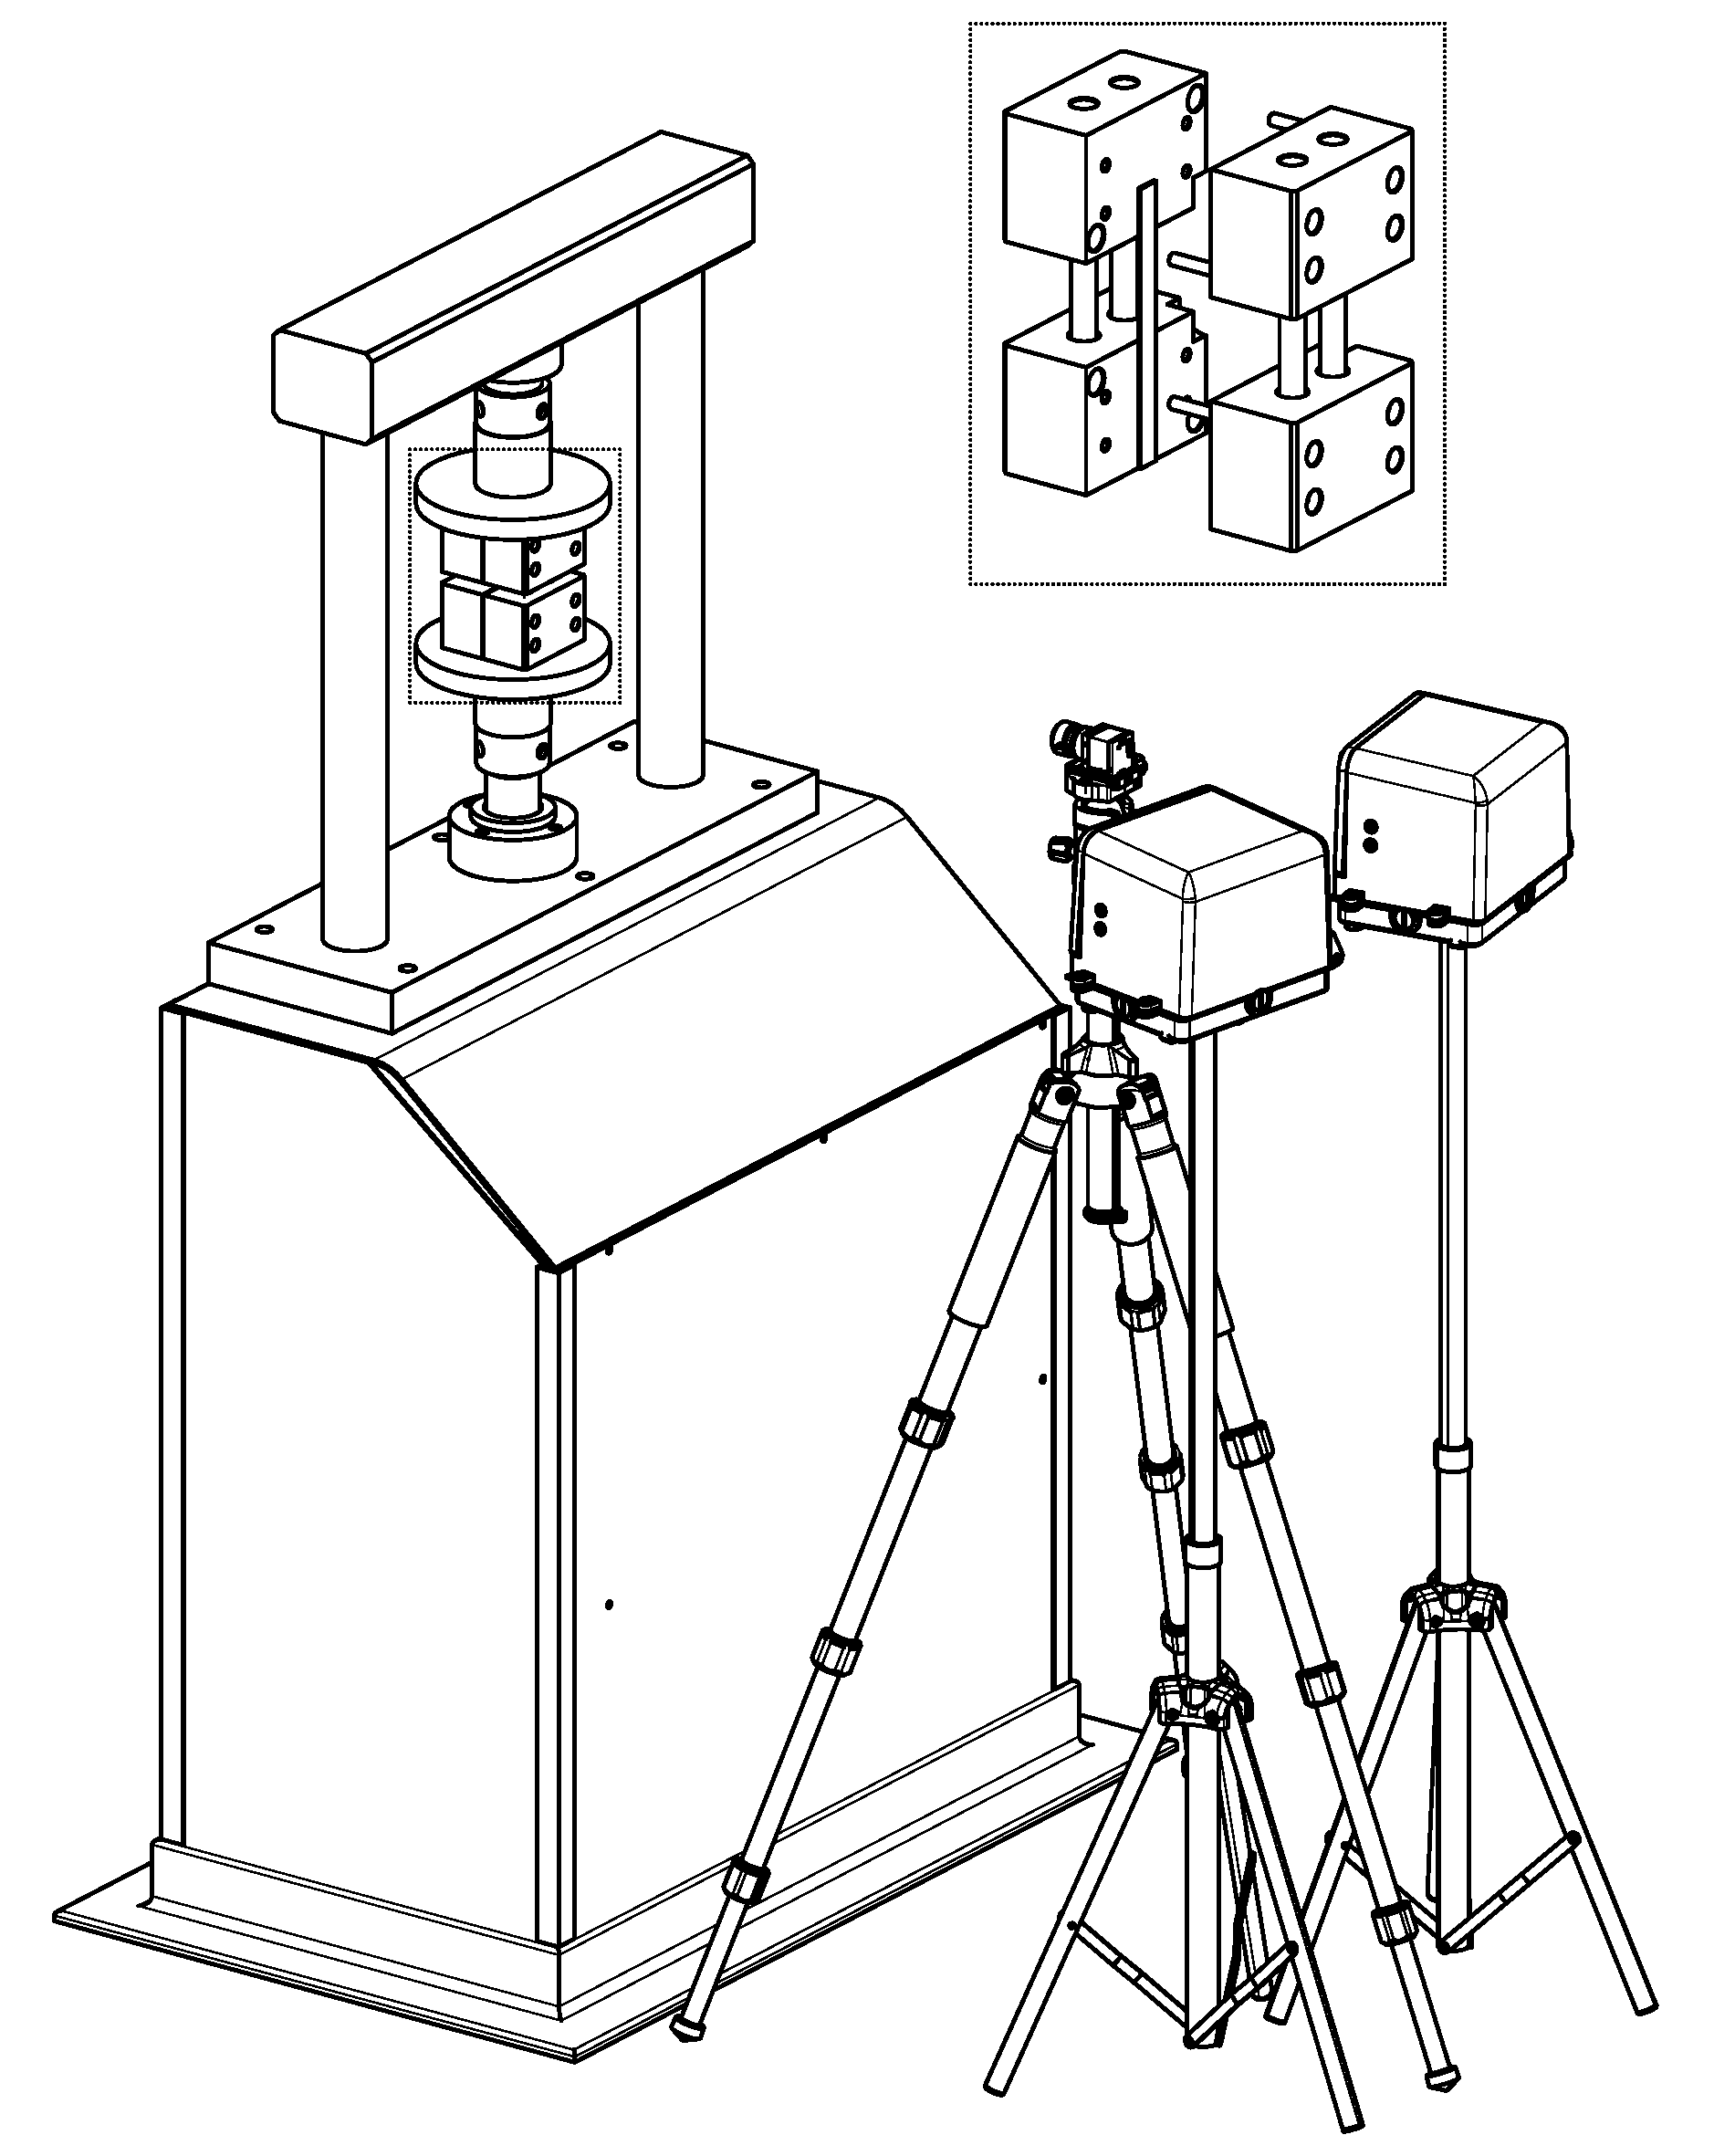
\includegraphics[scale=0.25]{\imgpath/\currfilebase/test_setup_scematic}
    \caption{Scematic of Test setup}
    \label{fig:test_setup_scematic}
\end{figure}

The test setup used consists of:
\begin{itemize}
    \item the test specimen
    \item a compressive test system generating and measuring displacement and load, where the load is measured using a $\SI{25}{\kilo\newton}$ load cell
    \item an anti-buckling test fixture, transmitting the load of the test system to the specimen
    \item a CCD camera setup with the camera itself, a lens and light sources mounted on tripods
    \item a PC with software that allows synced recording of the compressive test system and the CCD camera as well as DIC for post evaluation
\end{itemize}

Where the compressive test system used was an instron 8801 in displacement-controlled mode and the CLC test fixture in use was an ASTM D6641 similar to the one depicted in \autoref{fig:sketch_clc_fixture} but with four instead of two pillars in order to capture the strain field of the specimen. The clamping force of the fixture, acting on the specimen, is applied by increasing the torque of the clamping screws. The setup follows the recommendations of the test fixture standard \cite{D6641standard}.

\begin{figure}[!ht]
    \centering
    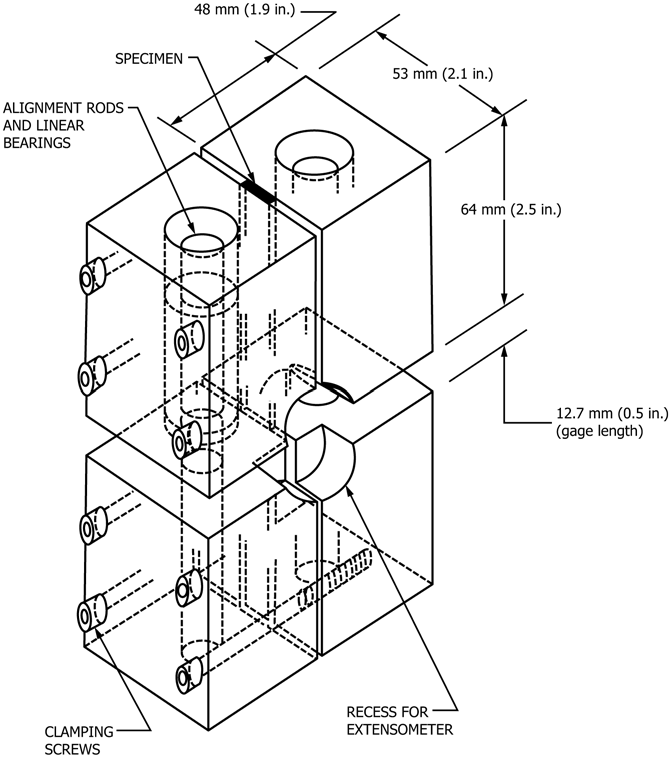
\includegraphics[scale=0.4]{\imgpath/\currfilebase/test_fixture.png}
    \caption{Dimensional Sketch of a Typical Combined Loading Compression (CLC) Test Fixture from \cite{D6641standard}}
    \label{fig:sketch_clc_fixture}
\end{figure}

\section{Specimen}
\label{sec:specimen}

The material used in the experiments is a unidirectional carbon fiber composite, i.e. a flat plate has been cured from thermoset prepregs\footnote{TC250 Resin System in unidirectional tape format} using pre-applied pressure of a vacuum bag and curing-pressure of an autoclave. The specimens were then shaped by water jet cutting this plate. An example cutting pattern is shown in \autoref{fig:specimen_plateA}, Where a bridge on each specimen circumference, connecting the base plate and the specimen, was not cut through to avoid the loss of specimens.
The Specimens were cut out in different angles with respect to the fiber direction. These angles are equal to the respective off-axis angles to the compressive loading direction in the setup if one neglects positioning inaccuracies.

For later identification, the specimens were labeled according to the test off-axis angle $\theta$, a plate identifier and a unique index.

\begin{figure}[!ht]
    \centering
    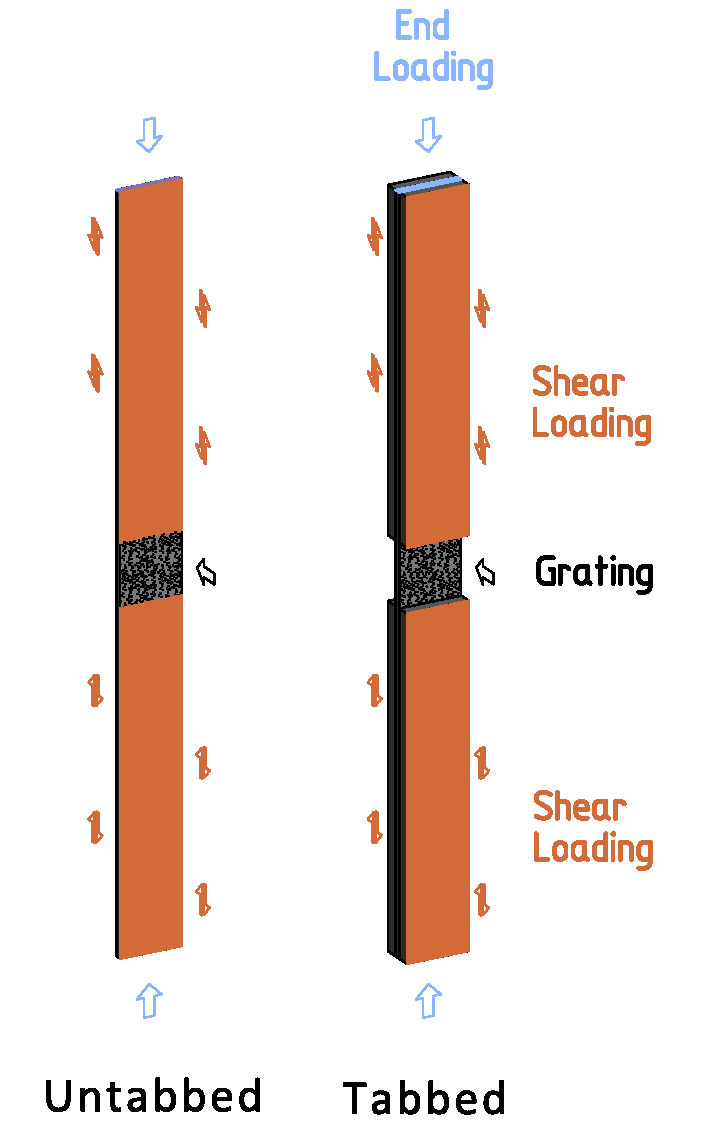
\includegraphics[scale=0.5]{\imgpath/\currfilebase/specimen_loads}
    \caption{Loads acting on both untabbed and tabbed specimens in setup respectively}
    \label{fig:specimen_loads}
\end{figure}
\begin{figure}[!ht]
    \centering
    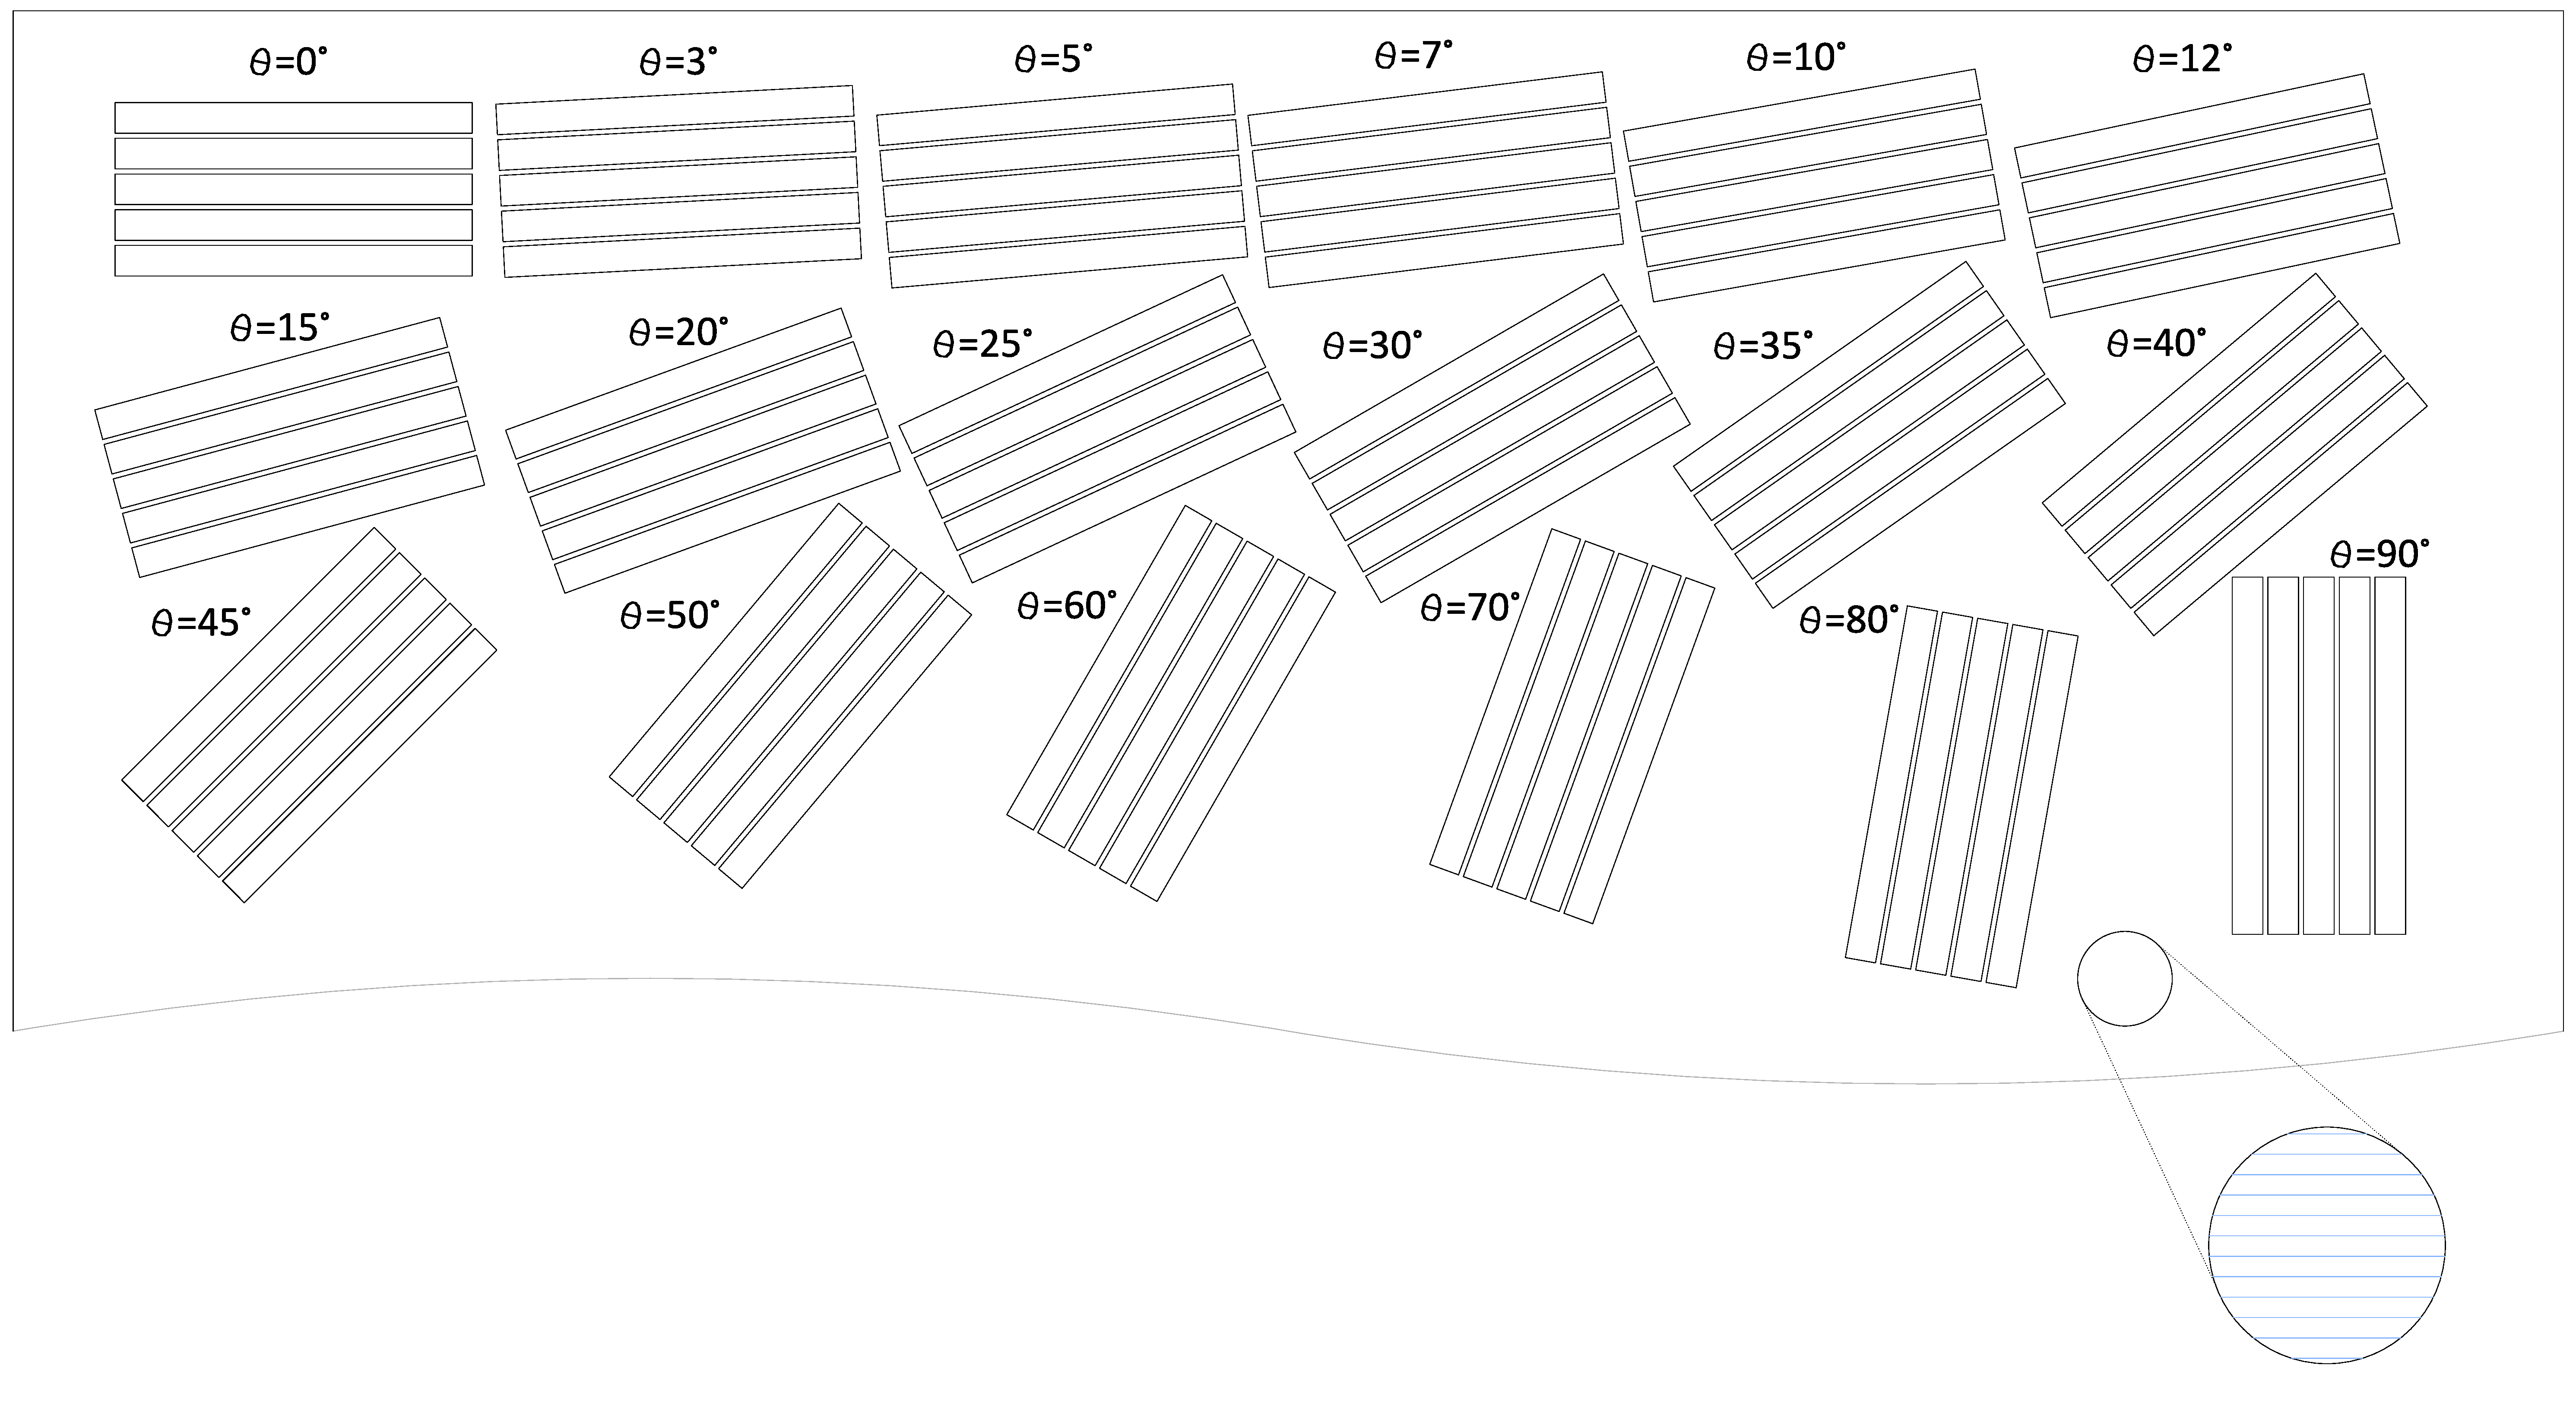
\includegraphics[scale=0.14]{\imgpath/\currfilebase/specimen_plateA}
    \caption{Water jet cutting pattern for carbon fiber plate with fiber direction indicated in blue and off-axis angle $\theta$}
    \label{fig:specimen_plateA}
\end{figure}

\newpage
\subsection{Specimen Preparation}
\label{subsec:spec_prep}

The specimen preparations include all alterations of the specimen after cutting the plate and before mounting it on the test setup. Specimens of both untabbed and tabbed form were tested on the test setup requiring different preparation steps.

\begin{minipage}[t]{\dimexpr(\distTextWidth-\distColSep)/2\relax}
    Untabbed specimen preparation:
    \begin{enumerate}
        \item Removing the specimens from the cut plate 
        \item Grinding off the remaining material from the connection to the base plate
        \item Roughening contact surface for fixture and grating
        \item Grating the field of interest at the mid-surface of the specimen
    \end{enumerate}
\end{minipage}% <- must be used if no gap
\hfill% <- use if there is a gap
\noindent
\begin{minipage}[t]{\dimexpr(\distTextWidth-\distColSep)/2\relax}
    Tabbed specimen preparation:
    \begin{enumerate}
        \item Removing the specimens and tabs from the cut plates respectively
        \item Grinding off the remaining material from the connection to the base plates for both the tabs and the specimen
        \item Roughening contact surfaces specimen tab connection and for fixture and grating
        \item Use adhesive bonding to connect the tabs to the specimens
        \item Grating the field of interest at the mid-surface of the specimen
    \end{enumerate}
\end{minipage}

\subsection{Specimen Dimensions}
\label{subsec:spec_dim}

The specimen dimensions follow the test fixture standard \cite{D6641standard}. The length of a specimen defines the gap between lower and upper part of the fixture at zero load. This gap was not varied in the scope of this thesis and has been chosen to be equal to the specimen width, i.e. it is small enough so that out-of-plane buckling is negligible. The resulting specimen dimensions are shown in \autoref{fig:specimen_nx_dim_labels}.

To be able to derive the compression stress from the compressive force one needs to devide it by the cross-section. Hence the cross-section must be known. Therefore the specimens were measured in both their thickness and width at multiple locations as depicted in \autoref{fig:specimen_nx_meas}.

\begin{figure}[!ht]
    \centering
    \begin{subfigure}[t]{\dimexpr(\distTextWidth-\distColSep)/2\relax}
        \centering
        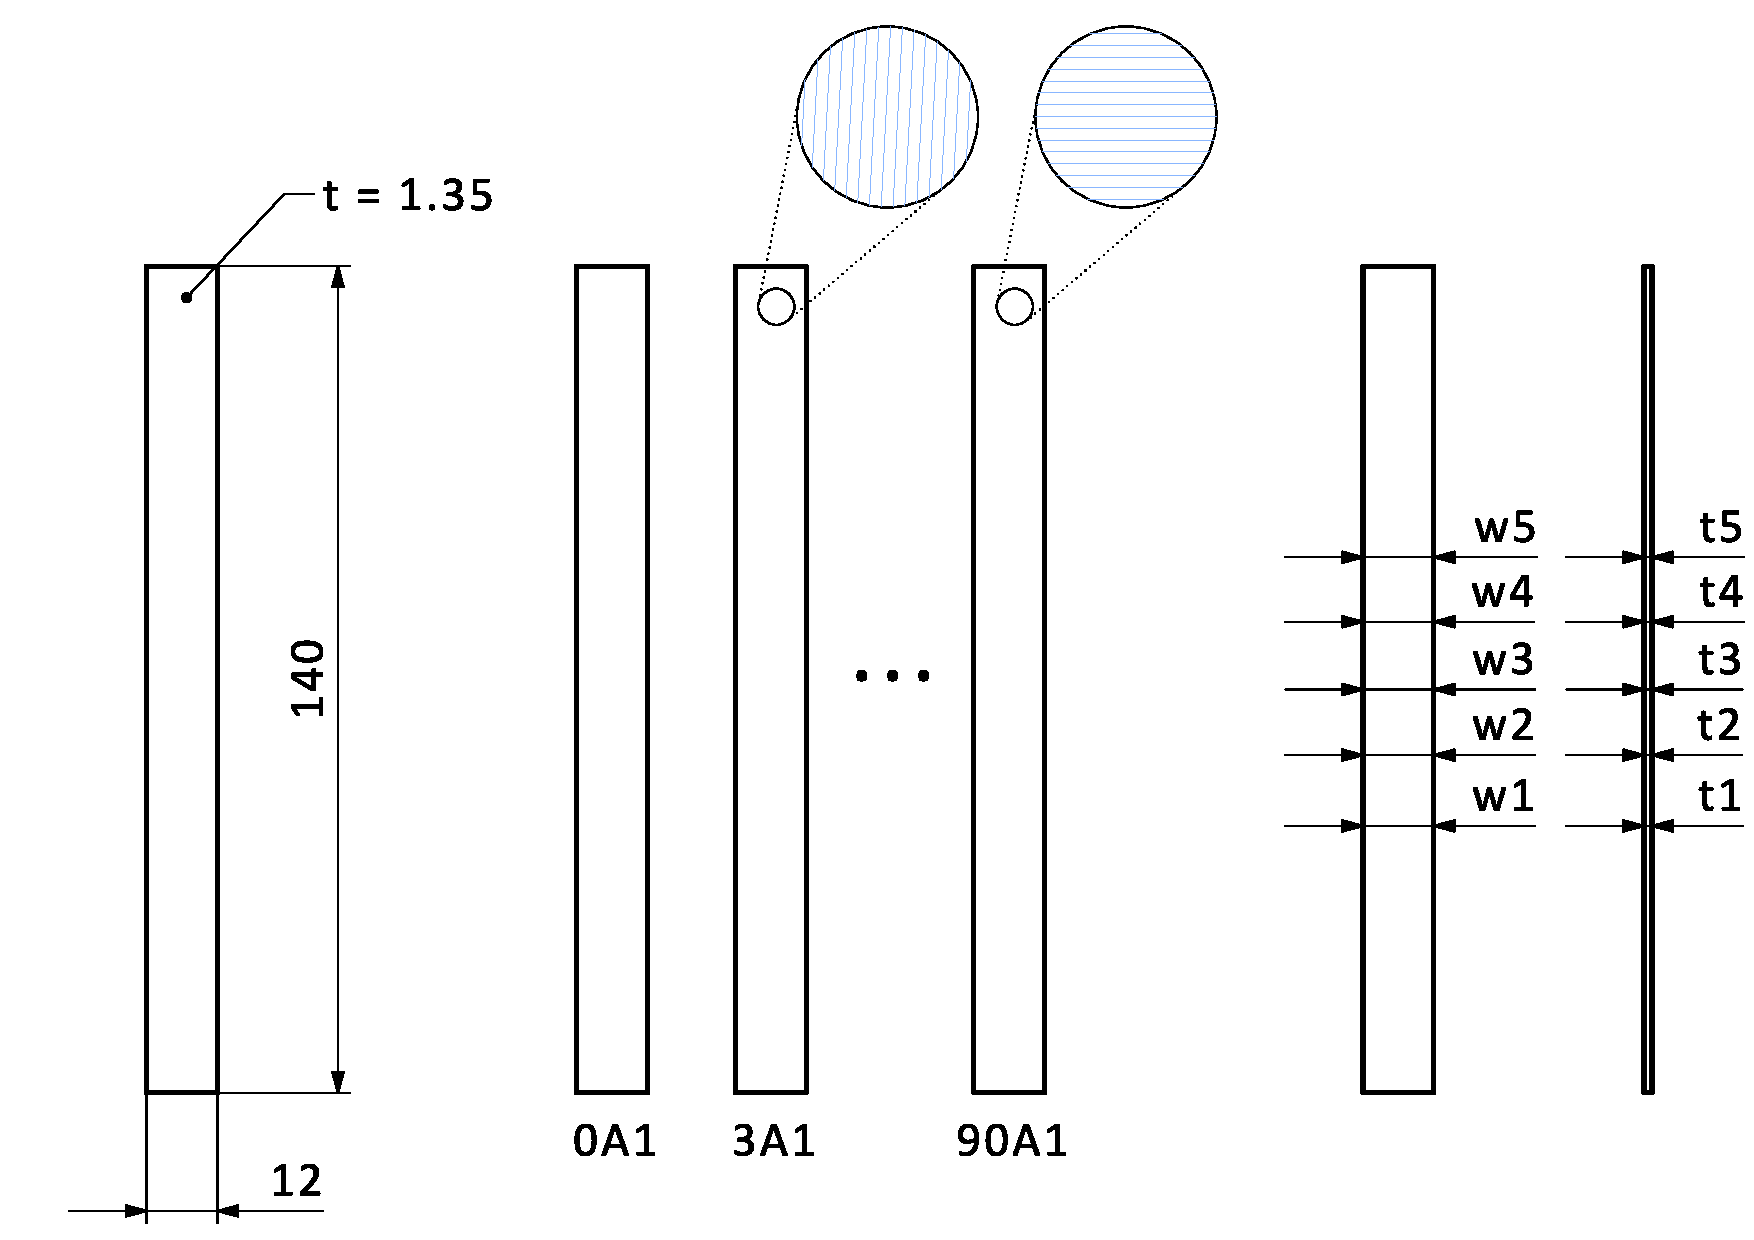
\includegraphics[%
        %trim={1cm 0.2cm 0cm 0.2cm}, % all views
        trim={1cm 0.2cm 9cm 0.2cm}, % dim and label
        %trim={1cm 0.2cm 21.5cm 3cm}, % dim
        %trim={9.5cm 1.5cm 9cm 0.2cm}, % label
        %trim={21.8cm 2.5cm 0cm 4.5cm}, % meas
        clip,scale=0.4]{\imgpath/\currfilebase/specimen}
        \caption{Specimen dimensions with example labels}
        \label{fig:specimen_nx_dim_labels}
    \end{subfigure}%
    \hfill
    \begin{subfigure}[t]{\dimexpr(\distTextWidth-\distColSep)/2\relax}
        \centering
        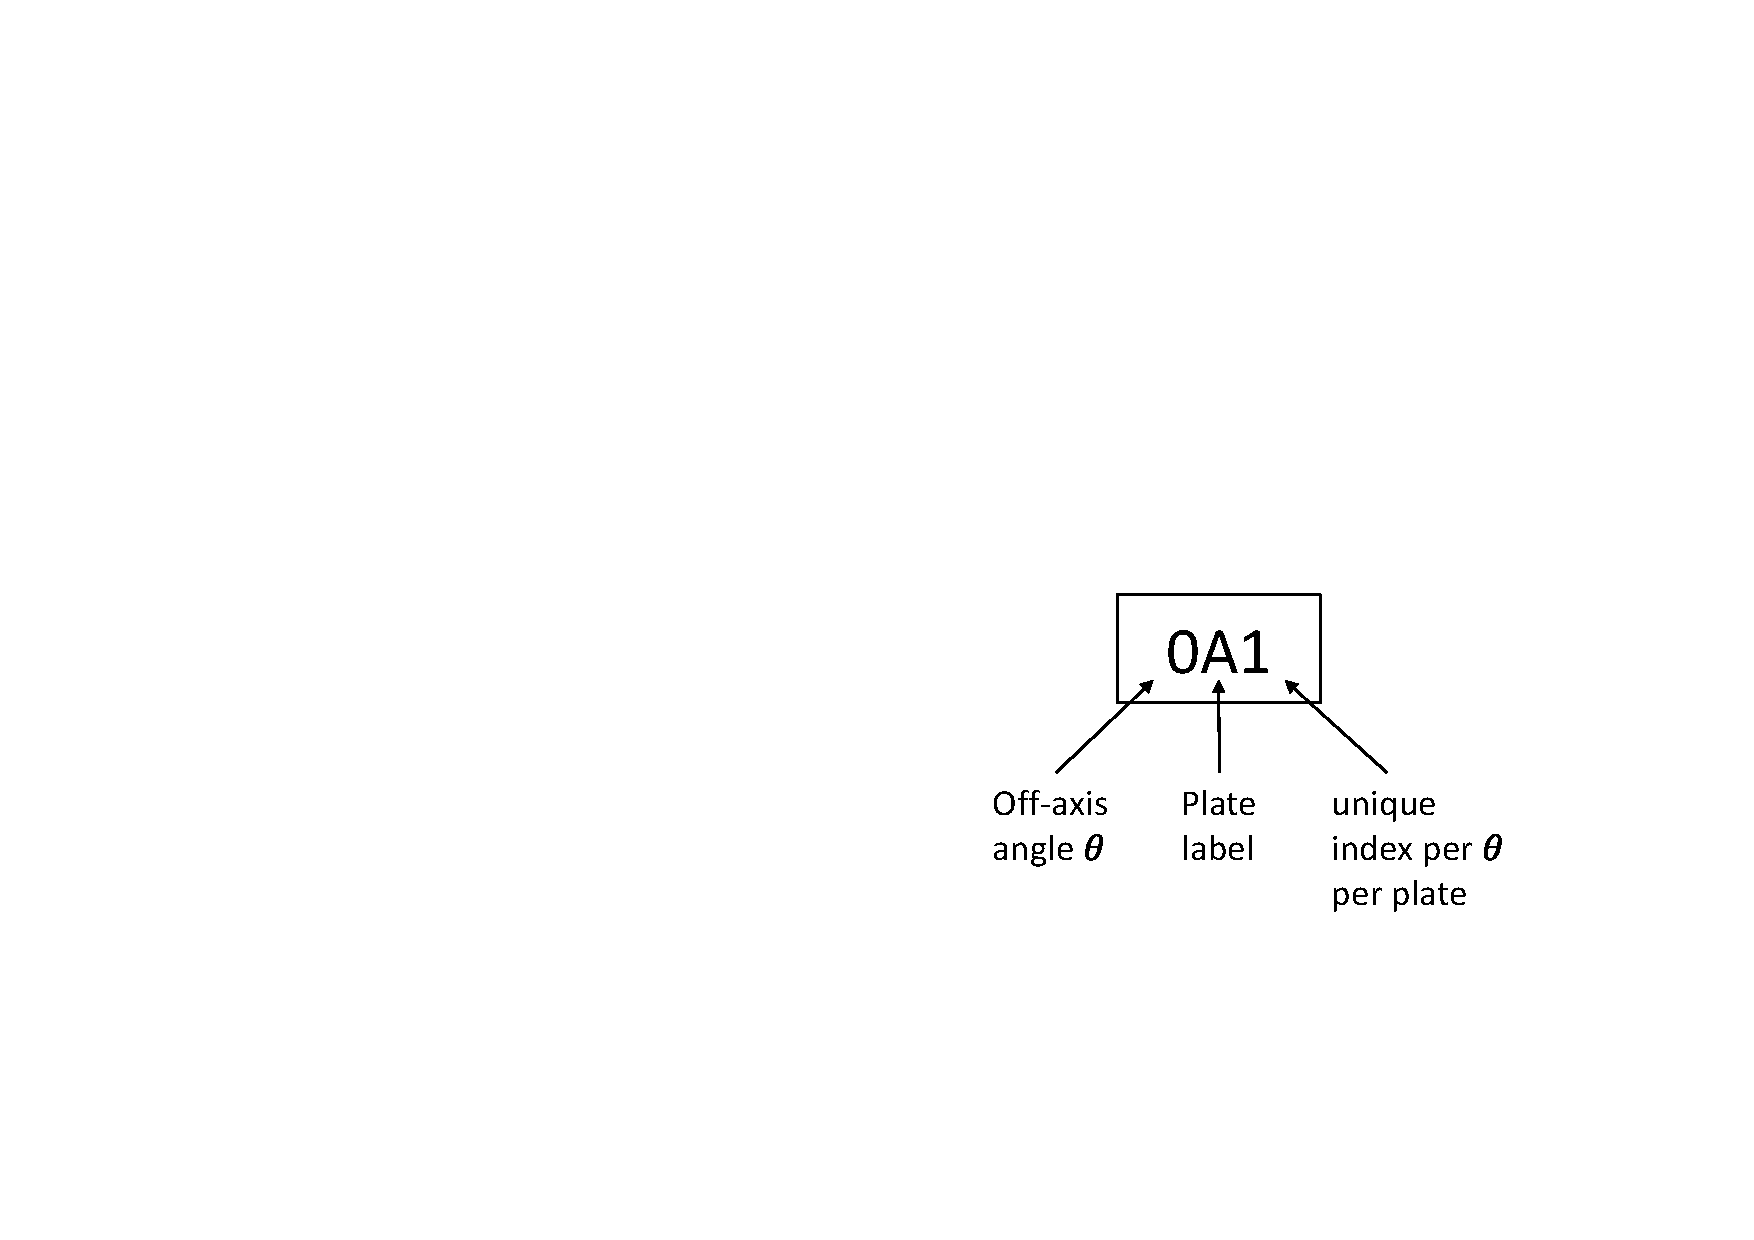
\includegraphics[scale=0.6]{\imgpath/\currfilebase/specimen_label}
        \caption{Specimen labelling system}
        \label{fig:specimen_label}
    \end{subfigure}
    \caption{Specimen dimensions and labels}
    \label{fig:specimen_dim_lab}
\end{figure}

\begin{figure}[!ht]
    \centering
    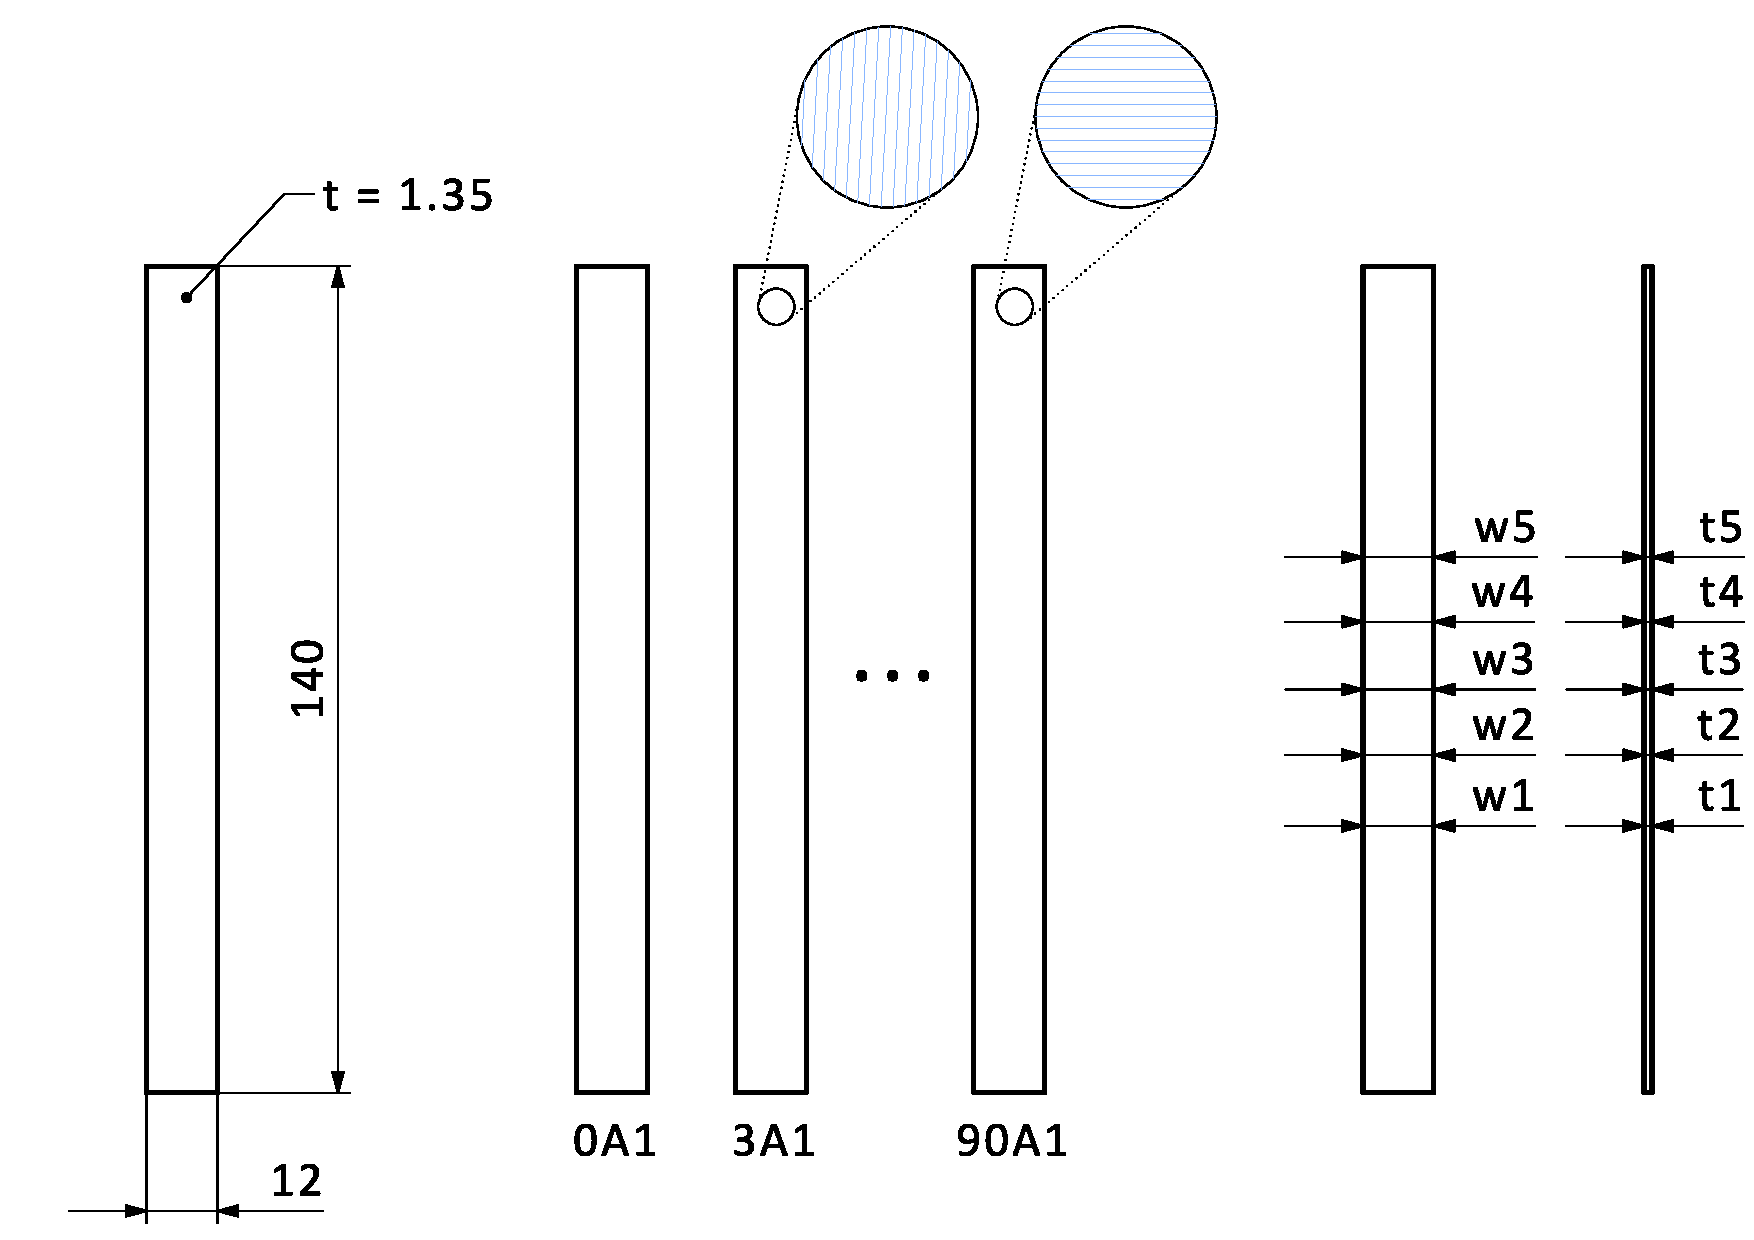
\includegraphics[%
    %trim={1cm 0.5cm 0cm 0.5cm}, % all views
    %trim={1cm 0.5cm 9cm 0.5cm}, % dim and label
    %trim={1cm 0.5cm 21.5cm 3cm}, % dim
    %trim={9.5cm 1.5cm 9cm 0.5cm}, % label
    trim={21.8cm 2.5cm 0cm 4.5cm}, % meas
    clip,scale=0.4]{\imgpath/\currfilebase/specimen}
    \caption{Specimen dimension measurements}
    \label{fig:specimen_nx_meas}
\end{figure}
\chapter{Preliminary Testing}
\label{chap:\currfilebase}

\section{Preliminary Testing Setup}
\label{sec:preliminary_testing_setup}

The preliminary tests were conducted on the setup described in \autoref{chap:test_setup} but without the use of any tabbed specimens. In terms of setup preparation The CLC fixture of the setup did not provide any means to position the specimen inside the fixture with good repeatably. However the off-axis angle of the fibre direction was the main parameter that has been exposed during experiments. Hence its accuracy and repeatability was important for reliable test results. For this reason a positioning device was 3D-printed from PLA to alleviate this issue. When assembling the fixture and specimen the positioning device is used as shown in \autoref{fig:fixture_positioner}.

\begin{figure}[!ht]
    \centering
    \begin{subfigure}[t]{\dimexpr(\distTextWidth-\distColSep)/2\relax}
        \centering
        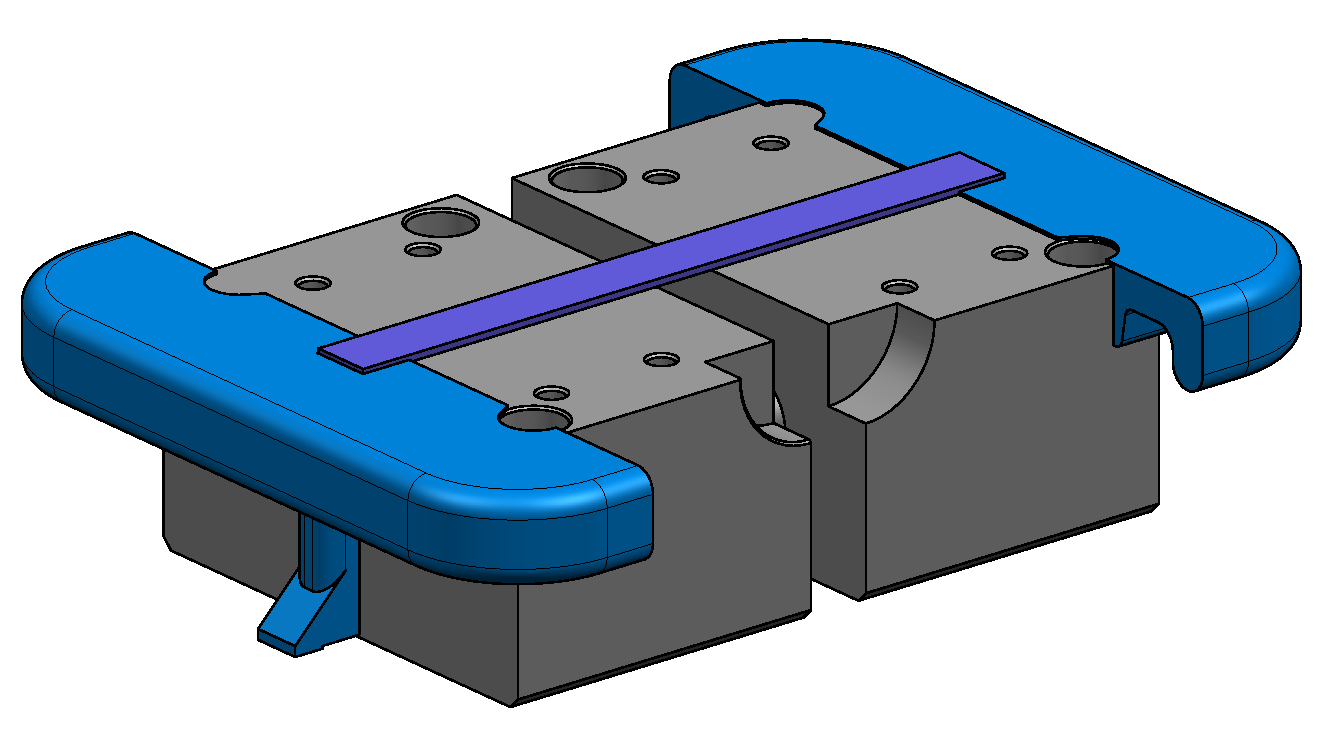
\includegraphics[scale=0.3]{\imgpath/\currfilebase/testfixture_positioner}
        \caption{untabbed specimen}
        \label{fig:fixture_positioner_untabbed}
    \end{subfigure}%
    \hfill
    \begin{subfigure}[t]{\dimexpr(\distTextWidth-\distColSep)/2\relax}
        \centering
        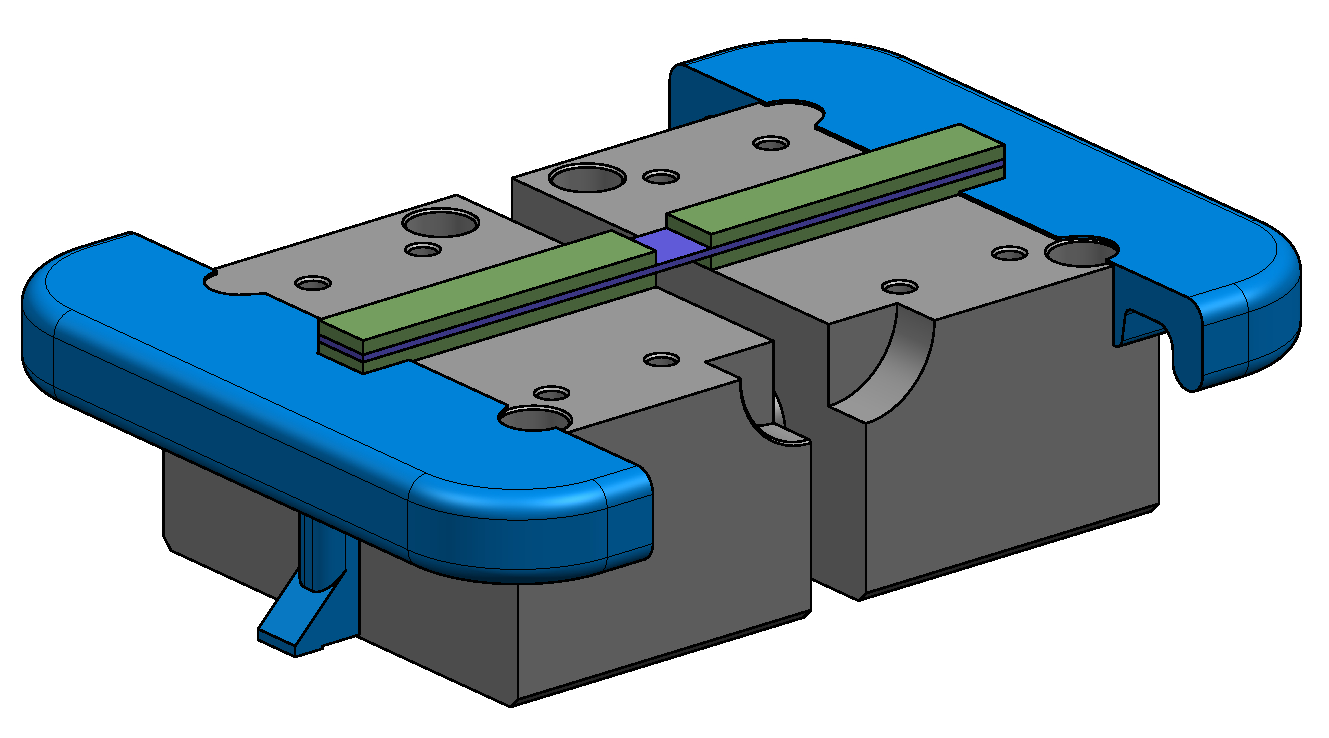
\includegraphics[scale=0.3]{\imgpath/\currfilebase/testfixture_positioner_tabbed}
        \caption{tabbed specimen}
        \label{fig:fixture_positioner_tabbed}
    \end{subfigure}
    \caption{3D-printed fixture positioner with specimen in violet, tabs in green, lower half of fixture in grey and fixture positioner in blue}
    \label{fig:fixture_positioner}
\end{figure}

\section{Preliminary Testing Results}
\label{sec:preliminary_testing_results}

In the preliminary testing specimens with off-axis below $\SI{20}{\degree}$ were prone to fail inside the fixture. This is an undesired use case since the CCD camera setup does not record the failure propagation and the compressive strength cannot be recorded with the desired accuracy. According to the fixture standard \cite{D6641standard} this is common for unidirectional lamina and can be counteracted by tabbing the specimens.

The torque of the clamping skrews of the test fixture had a significant impact on the absolute compressive stress at failure. To counteract this variance the clamping skrews were fastened with a torque wrench, using the limit of $\SI{5}{\newton\meter}$ for most experiments.

\section{Tabbing Process}
\label{sec:tabbing_process}

Tabbed specimens were to be positioned by the same positioning device as untabbed ones, see \autoref{fig:fixture_positioner_tabbed}. Thus the tabbing process had to fulfill a high accuracy, so that the off-axis angle was reached with an equally good repeatably. Hence a 3D-printed tab positioner was used for aligning tabs and specimen during the adhesive bonding. The parts were assembled on pins as shown in \autoref{fig:tab_fixture_ass}.

\begin{figure}[!ht]
    \centering
    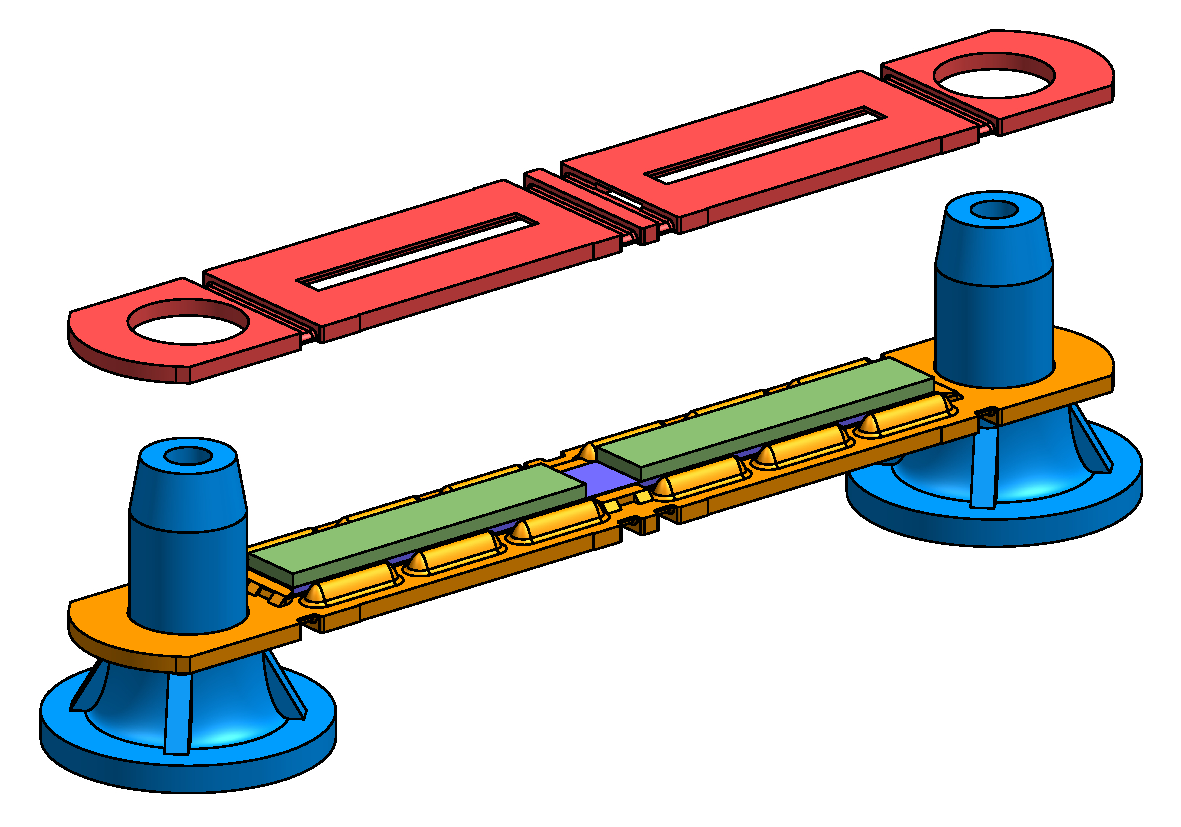
\includegraphics[scale=0.6]{\imgpath/\currfilebase/tab_fixture}
    \caption{Tabbing fixture assembly}
    \label{fig:tab_fixture_ass}
\end{figure}
\chapter{Experimental Results}
\label{chap:\currfilebase}
...

\begin{figure}[!ht]
    \centering
    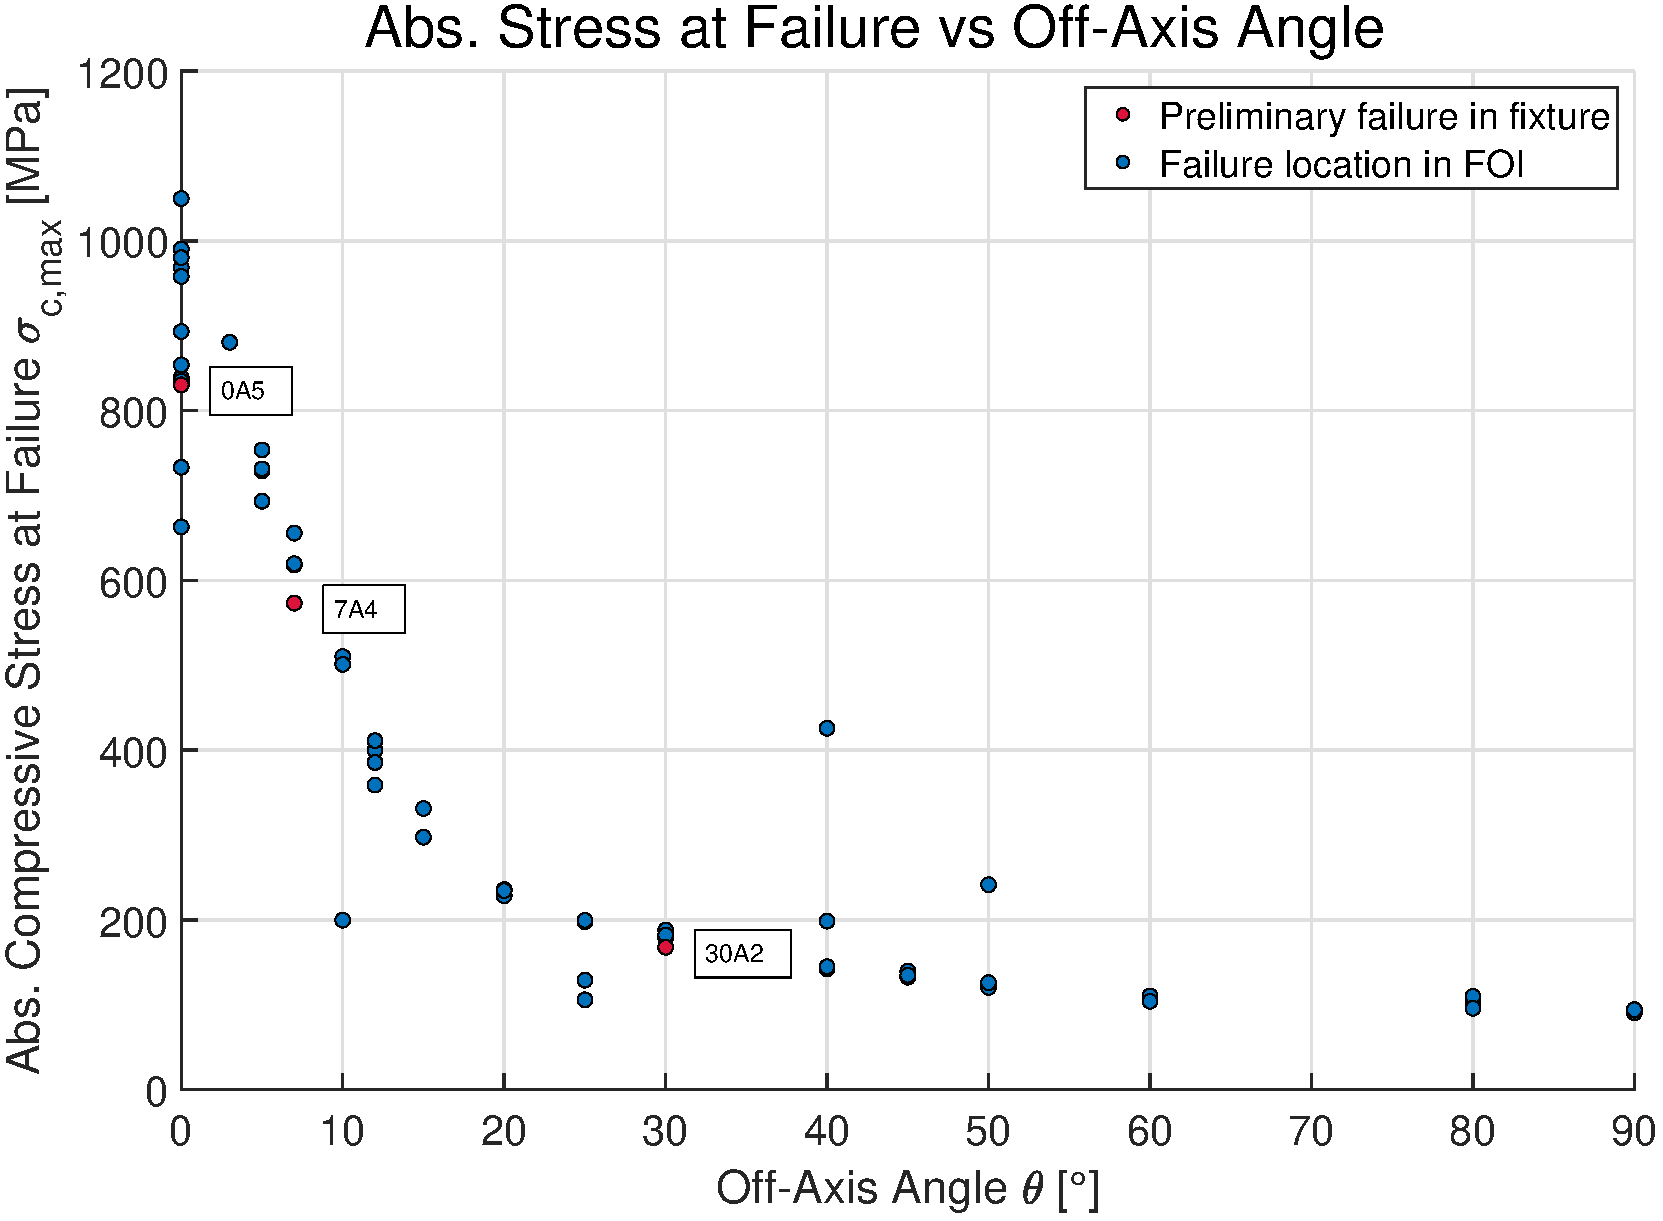
\includegraphics[scale=0.4]{\imgpath/\currfilebase/Strength_OffAngle_1.pdf}
    \caption{Abs. compressive stress at failure over off axis angle, all measurements}
    \label{fig:strength_offAngle_1}
\end{figure}
\begin{figure}[!ht]
    \centering
    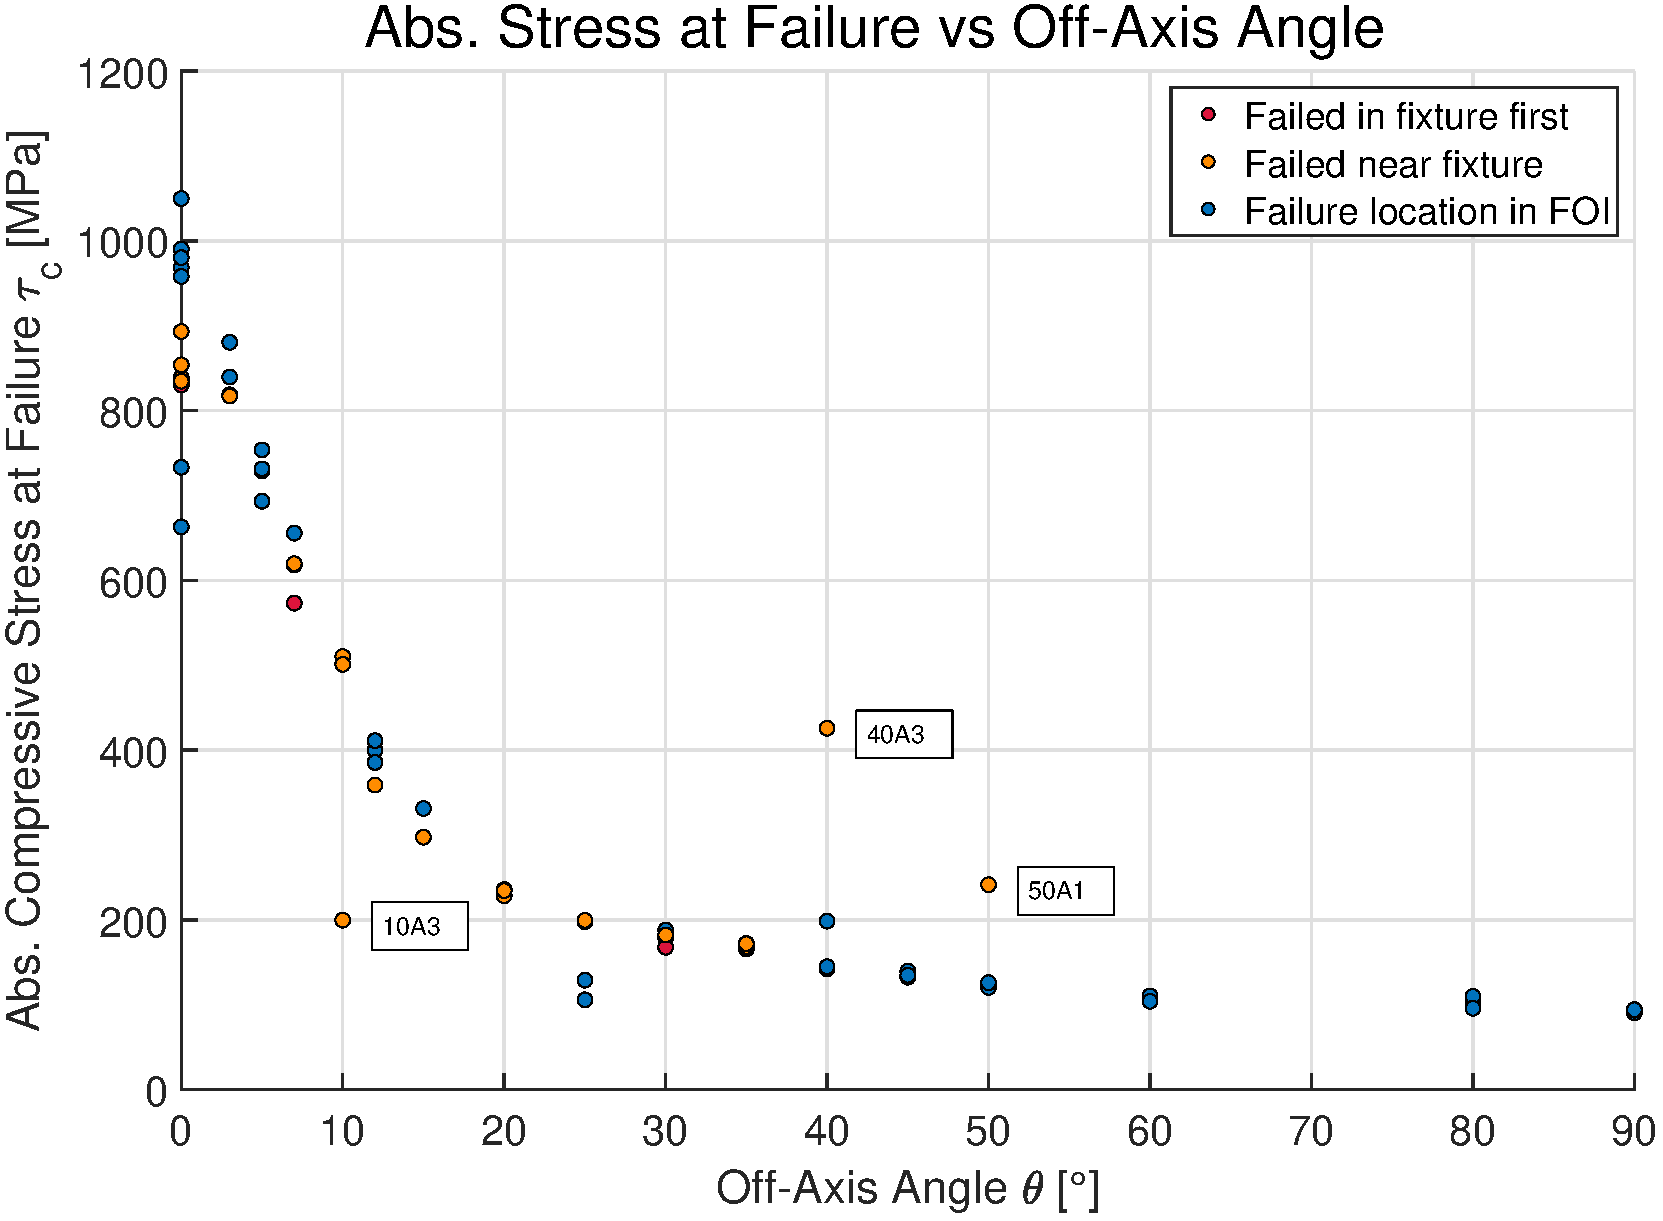
\includegraphics[scale=0.4]{\imgpath/\currfilebase/Strength_OffAngle_2.pdf}
    \caption{Abs. compressive stress at failure over off axis angle, \#2}
    \label{fig:strength_offAngle_2}
\end{figure}
\begin{figure}[!ht]
    \centering
    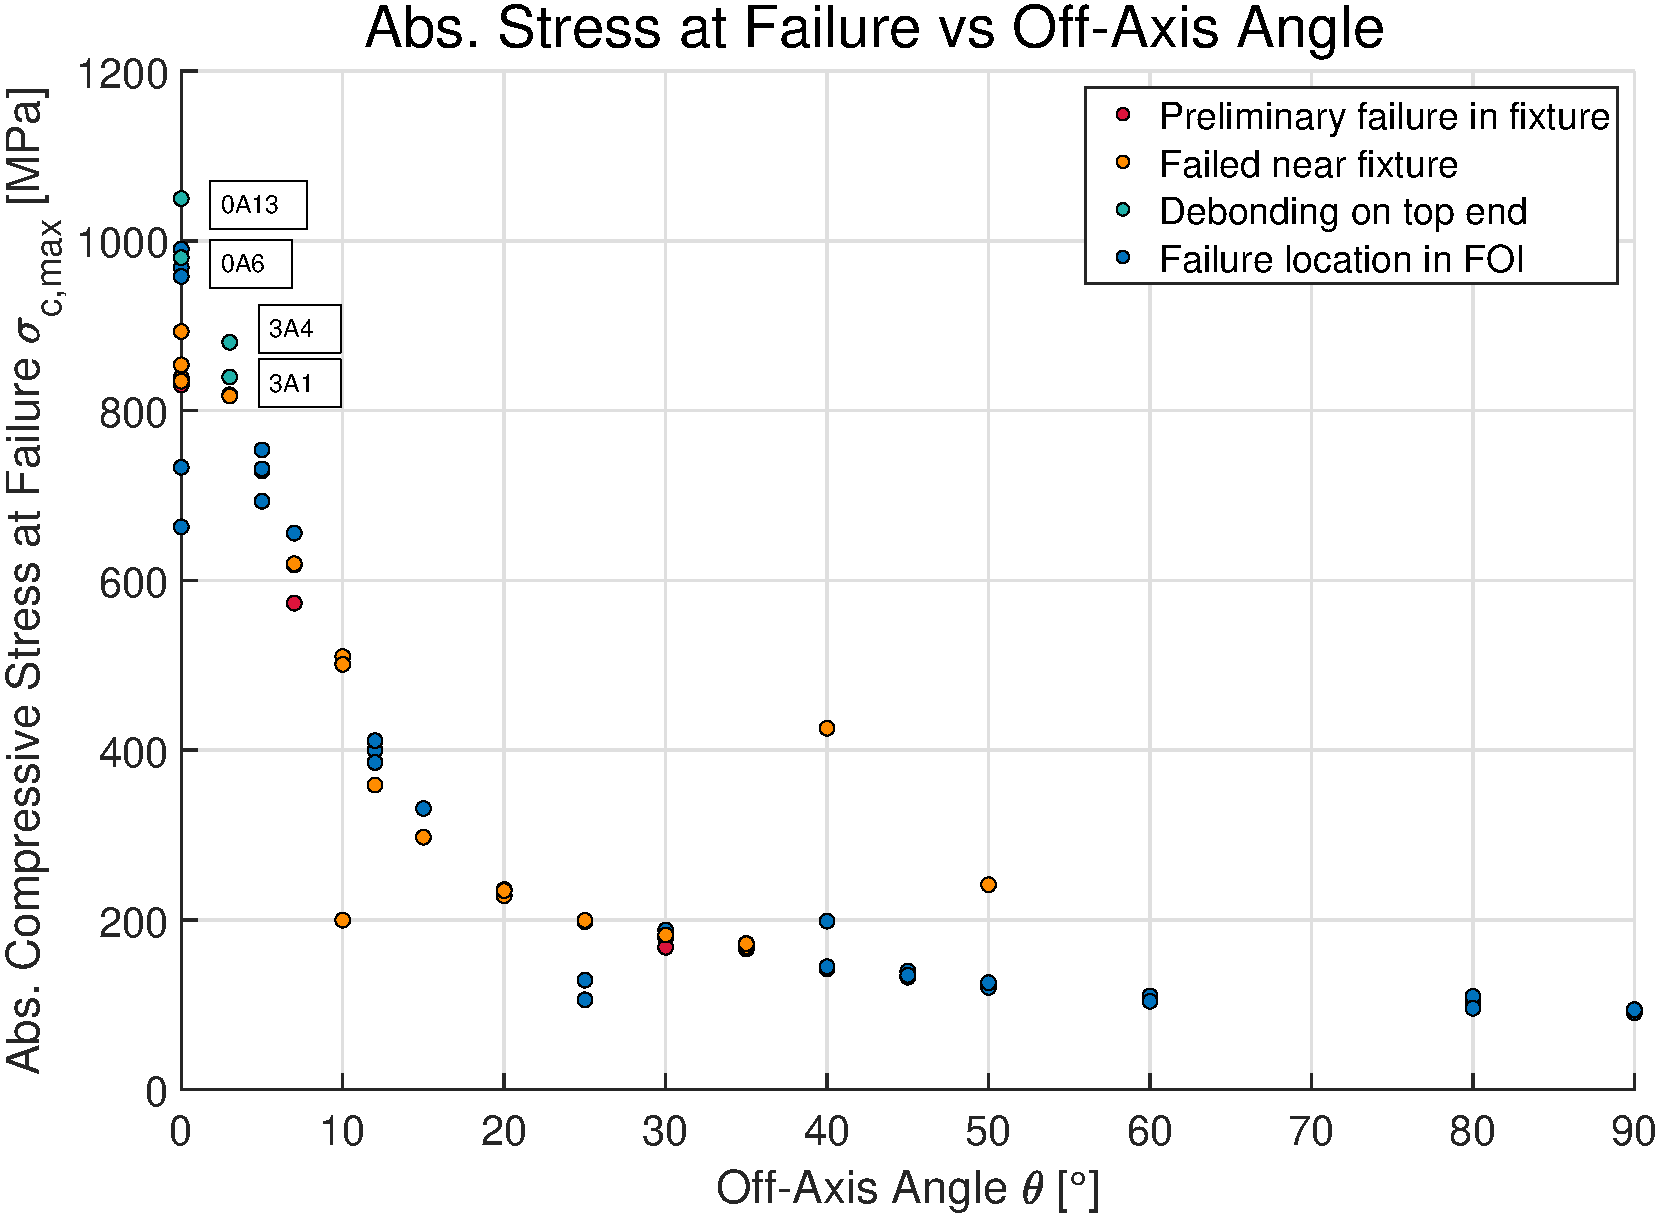
\includegraphics[scale=0.4]{\imgpath/\currfilebase/Strength_OffAngle_3.pdf}
    \caption{Abs. compressive stress at failure over off axis angle, \#3}
    \label{fig:strength_offAngle_3}
\end{figure}
\begin{figure}[!ht]
    \centering
    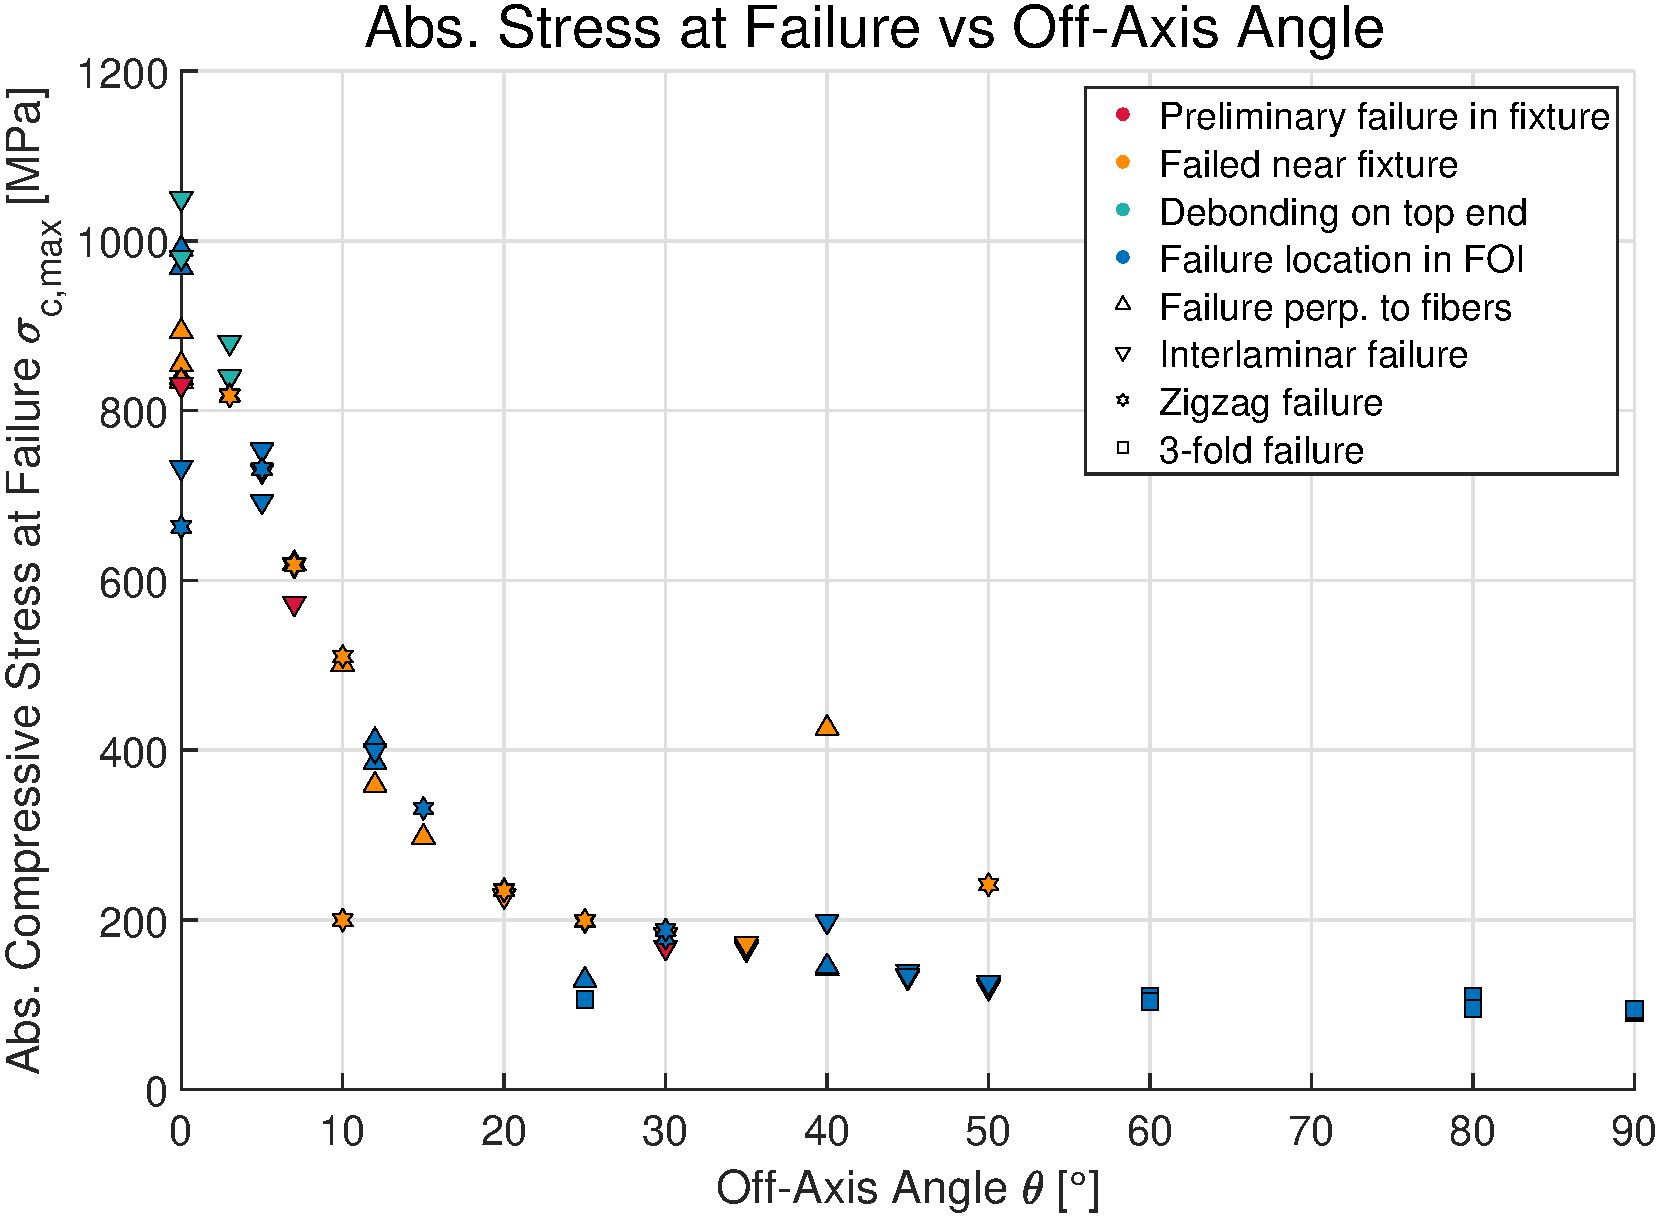
\includegraphics[scale=0.4]{\imgpath/\currfilebase/Strength_OffAngle_4.pdf}
    \caption{Abs. compressive stress at failure over off axis angle, \#4}
    \label{fig:strength_offAngle_4}
\end{figure}
\begin{figure}[!ht]
    \centering
    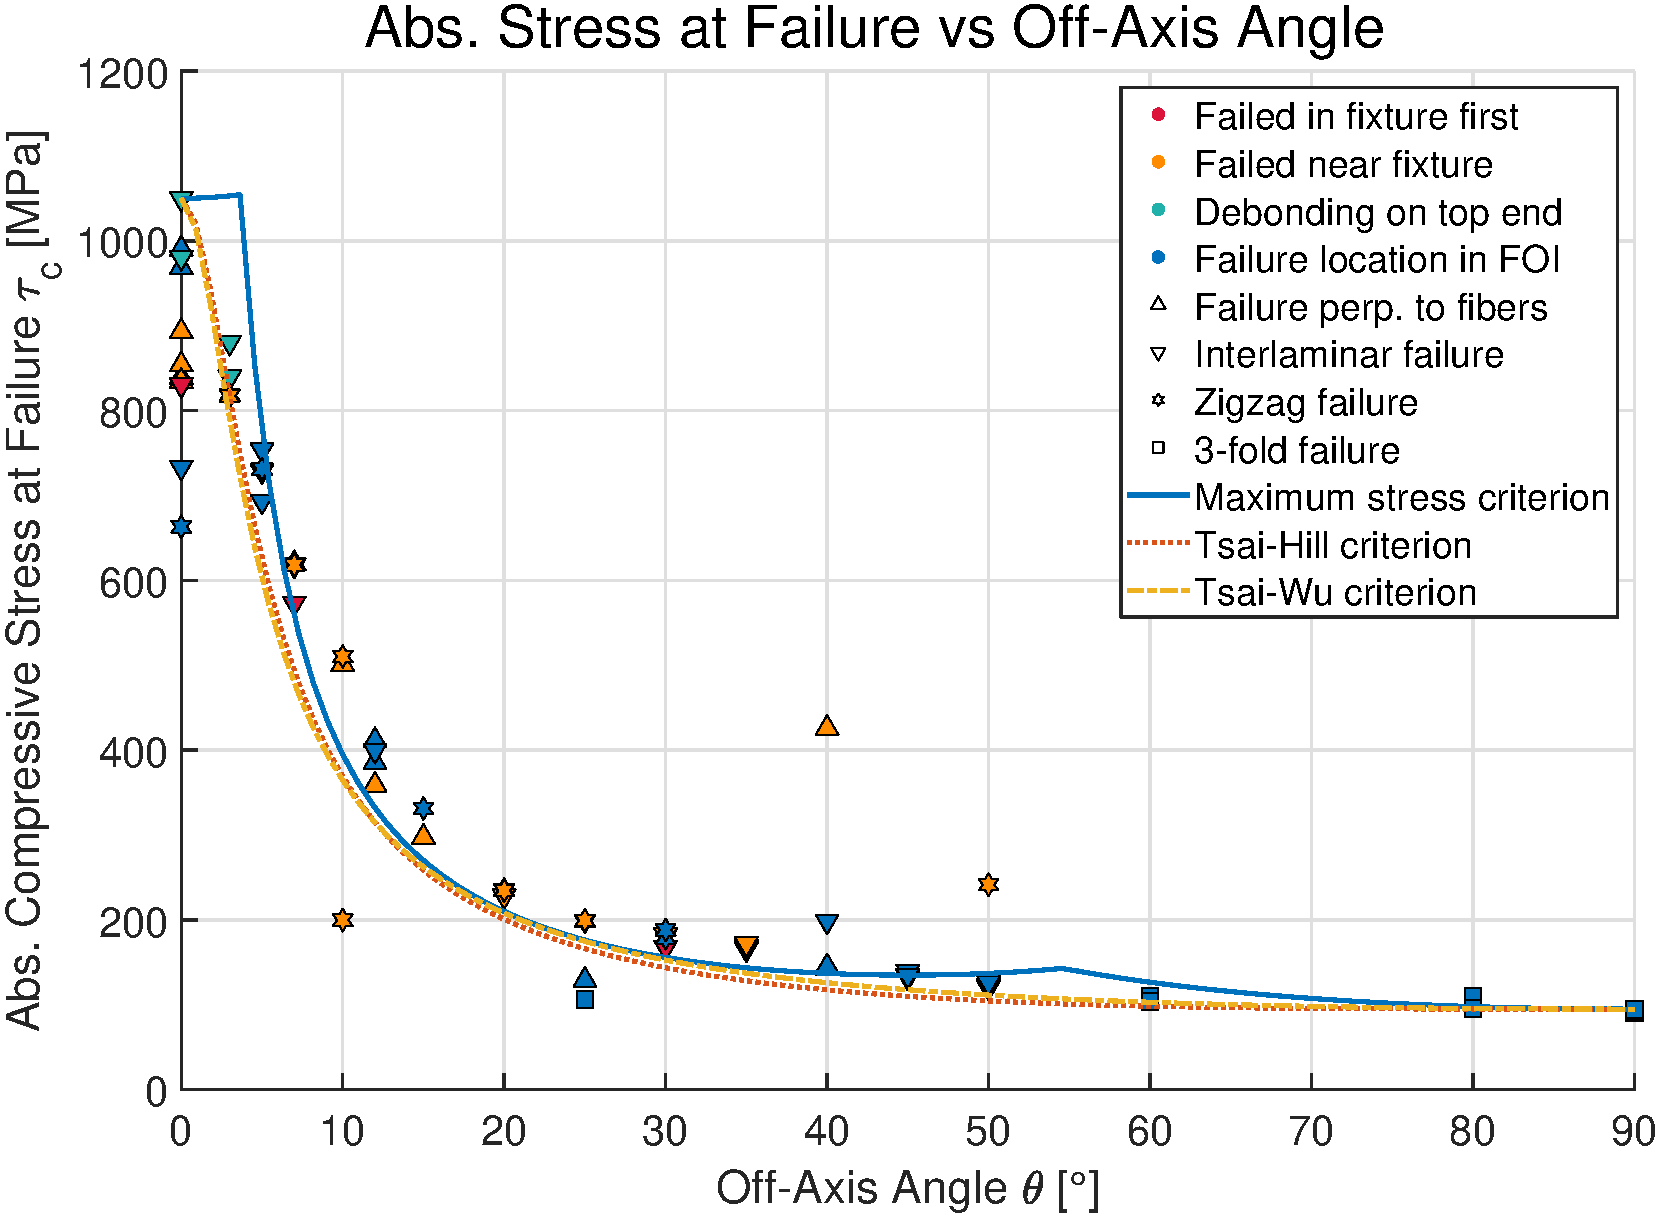
\includegraphics[scale=0.4]{\imgpath/\currfilebase/Strength_OffAngle_5.pdf}
    \caption{Abs. compressive stress at failure over off axis angle, \#5}
    \label{fig:strength_offAngle_5}
\end{figure}
% The following measurement results are represented as the positioning error motions of the different target point over time, the relevant temperature over time and a surface plot of the positioning error motions relative to the first positioning error motion over time and target point position. Where the later aims to show the deviations neglecting their geometrical error contribution.\par
% Straightness error motions are not addressed since their deviations lie within the measurement uncertainty of the position measuring instrument.\par
% All measurement results shown in this thesis are conducted using the measurement head of the linear encoder itself (Figure~{\ref{fig:heidenhainvm182_3d}}). Measurement results using another scanning head are left out as they cannot be compared with the ones listed. 
% Additional measurement results can be found in the appendix.
% \newpage

% \section{Cold test\label{sec:resultcold}}

% %appendix: cold test 17112017 n_t=140

% \subsection*{Observations in a cold test over three days}
% In Figure~{\ref{fig:coldtest_24112017_devtemp}} the positioning error motion of the individual target points and different temperatures of importance are depicted over time. The positioning error motions of the individual target points show a similar curvature with respect to each other but have different initial values. All temperature curvatures follow the same pattern but with different magnitudes of the deflections. One may notice the contemporaneous deflections of the negative positioning error motion and environmental temperature especially at temperature peaks. When considering the relative positioning error motion as depicted in Figure~{\ref{fig:coldtest_24112017_surf}}, it becomes apparent that the time dependant deviation range remains below {\SI{3}{\micro\metre}} for all target points alike.
% \newpage

% \begin{figure}[H]
% \centering
% \includegraphics[width=0.85\linewidth]{figures/measurementresults/cold/coldtest_24112017_devtemp}
% \caption[Positioning error motions motions and relevant temperatures cold 24.11.2017]{Positioning error motions and relevant temperature profiles over time of the cold test started on November 24th 2017. Setting parameter $n_t=140$}
% \label{fig:coldtest_24112017_devtemp}
% \end{figure}
% \vspace{2\baselineskip}
% \begin{figure}[H]
% \centering
% \includegraphics[width=0.85\linewidth]{figures/measurementresults/cold/coldtest_24112017_surf}
% \caption[Relative positioning error motion cold 24.11.2017]{Relative positioning error motion of the cold test started on November 24th 2017. Setting parameter $n_t=140$}
% \label{fig:coldtest_24112017_surf}
% \end{figure}
% %---
% \newpage

% %----------------------------------------------------------------------
% \section{Warm-Cold test\label{sec:resultwarmcold}}

% %appendix: warmcoldtest 07112017 v_w=5000
% %appendix: warmcoldtest 10112017 v_w=12500 special test

% \subsection*{Observations in a warm-cold test with an oscillation feed rate of 12500 mm/min}
% As previously seen in a cold test (Section~{\ref{sec:resultcold}}) the positioning error motions over time of the different target point show a similar pattern with respect to each other but start at increasing initial values (Figure~{\ref{fig:warmcoldtest_11112017a_devtemp}}). A distinct effect that can be observed in a warm-cold test is the rise in the temperatures of the Y-axis spindle motor and the spindle nut during the first phase of the test. Those temperatures both rise until a saturation temperature is reached in the warm phase and approximate the the environmental temperature in the cold phase while relating to lead-lag properties. Especially when considering the relative positioning error in Figure~{\ref{fig:warmcoldtest_11112017a_surf}} the very same lead-lag properties may be identified in the negative of the deviations. The range of the relative positioning error motions over time remains similar compared to a cold test.
% \newpage

% \begin{figure}[H]
% \centering
% \includegraphics[width=0.85\linewidth]{figures/measurementresults/warmcold/warmcoldtest_11112017a_devtemp}
% \caption[Positioning error motions motions and relevant temperatures warm-cold 11.11.2017a]{Positioning error motions and relevant temperature profiles over time of the warm-cold test started on November 11th 2017. Setting parameter $v_w=\SI{12500}{\mm\per\minute}$}
% \label{fig:warmcoldtest_11112017a_devtemp}
% \end{figure}
% \vspace{2\baselineskip}
% \begin{figure}[H]
% \centering
% \includegraphics[width=0.85\linewidth]{figures/measurementresults/warmcold/warmcoldtest_11112017a_surf}
% \caption[Relative positioning error motion warm-cold 11.11.2017a]{Relative positioning error motion of the warm-cold test started on November 11th 2017. Setting parameter $v_w=\SI{12500}{\mm\per\minute}$}
% \label{fig:warmcoldtest_11112017a_surf}
% \end{figure}
% %---
% \newpage

% \subsection*{Observations in a warm-cold test with an oscillation feed rate of 5000 mm/min}
% In this warm-cold test the same behaviour as in warm-cold tests with higher feed rate of oscillations, as in Figure~{\ref{fig:warmcoldtest_11112017a_devtemp}} occurs. The difference lies in the impact of the warm-phase on the temperatures and deviations. The saturation temperature of the temperature curvatures showing lead-lag properties is lower in a test with smaller oscillation feed rate (See Figure~{\ref{fig:warmcoldtest_10112017b_devtemp}}). Furthermore the negative of the relative positioning error motions depict less lead-lag properties (Figure~{\ref{fig:warmcoldtest_10112017b_surf}}).

% \begin{figure}[H]
% \centering
% \includegraphics[width=0.85\linewidth]{figures/measurementresults/warmcold/warmcoldtest_10112017b_devtemp}
% \caption[Positioning error motions motions and relevant temperatures warm-cold 10.11.2017b]{Positioning error motions and relevant temperature profiles over time of the warm-cold test started on November 10th 2017. Setting parameter $v_w=\SI{5000}{\mm\per\minute}$}
% \label{fig:warmcoldtest_10112017b_devtemp}
% \end{figure}
% \vspace{2\baselineskip}
% \begin{figure}[H]
% \centering
% \includegraphics[width=0.85\linewidth]{figures/measurementresults/warmcold/warmcoldtest_10112017b_surf}
% \caption[Relative positioning error motion warm-cold 10.11.2017b]{Relative positioning error motion of the warm-cold test started on November 10th 2017. Setting parameter $v_w=\SI{5000}{\mm\per\minute}$}
% \label{fig:warmcoldtest_10112017b_surf}
% \end{figure}
% %---
% \newpage

% %appendix: warmcoldtest 11112017, v_w=5000
% %appendix: warmcoldtest 16112017, v_w=3000
% %appendix: warmcoldtest 20112017oil, v_w=3000
% %appendix: warmcoldtest 23112017, v_w=6000
% %appendix: warmcoldtest 27112017, v_w=12500
% %appendix: warmcodltest 07122017, v_w=3000

% %----------------------------------------------------------------------
% \section{Multi-range test\label{sec:resultmultirange}}

% %appendix: multirangetest 08122017
% %appendix: multirangetest 10122017
% %appendix: mulitrangetest 16122017

% \subsection*{Observations in a multi-range test with an oscillation feed rate of 12500 mm/min and three different oscillation starting points}
% Although in a multi-range test the position of oscillation is changed after each warm phase, there is not a significant difference in the measurement results when compared to a warm-cold test (Section~{\ref{sec:resultwarmcold}}). Apparent is the larger range of deviation over time of more than {\SI{7}{\micro\metre}} (See Figure~{\ref{fig:multirangetest_14122017_surf}}) which can be lead back to MT warm-up effects. But namely the positioning error motion of the different target points with respect to each other does not change noticeably over time with exception of the first three hours during MT warm-up (Figure~{\ref{fig:multirangetest_14122017_devtemp}}) compared to a warm-cold test with the same oscillation feed rate (example given Figure~{\ref{fig:warmcoldtest_11112017a_devtemp}}).
% \newpage

% \begin{figure}[H]
% \centering
% \includegraphics[width=0.85\linewidth]{figures/measurementresults/multirange/multirangetest_14122017_devtemp}
% \caption[Positioning error motions motions and relevant temperatures multi-range 14.12.2017]{Positioning error motions and relevant temperature profiles over time of the multi-range test started on December 14th 2017. Setting parameter $v_w=\SI{12500}{\mm\per\minute}$, $l_{s,1}=\SI{0}{\mm}$, $l_{s,2}=\SI{100}{\mm}$ and $l_{s,3}=\SI{200}{\mm}$}
% \label{fig:multirangetest_14122017_devtemp}
% \end{figure}
% \vspace{2\baselineskip}
% \begin{figure}[H]
% \centering
% \includegraphics[width=0.85\linewidth]{figures/measurementresults/multirange/multirangetest_14122017_surf}
% \caption[Relative positioning error motion multi-range 14.12.2017]{Relative positioning error motion of the multi-range test started on December 14th 2017. Setting parameter $v_w=\SI{12500}{\mm\per\minute}$, $l_{s,1}=\SI{0}{\mm}$, $l_{s,2}=\SI{100}{\mm}$ and $l_{s,3}=\SI{200}{\mm}$}
% \label{fig:multirangetest_14122017_surf}
% \end{figure}
% %---
% \newpage


% %----------------------------------------------------------------------
% \section{Stairs test\label{sec:resultstairs}}

% \subsection*{Observations in a stairs test with an oscillation feed rate of 12500 mm/min}
% The alternation of warm and cold phases is accelerated in a stairs test compared to a warm-cold test. here in this specific test five warm phases and cold phases are altered respectively in an up and down configuration respectively (See Section~{\ref{sec:stairstest}}). When focusing on the negative of the relative positioning error motions in Figure~{\ref{fig:stairstest_12112017_surf}} the adaptation of lead-lag properties of the deviation derived of the temperatures in Figure~{\ref{fig:stairstest_12112017_devtemp}} is confirmed. Bare in mind that the deflections of the positioning error motions are contemptuous with the temperatures that show lead-lag properties.
% \newpage

% \begin{figure}[H]
% \centering
% \includegraphics[width=0.85\linewidth]{figures/measurementresults/stairs/stairstest_12112017_devtemp}
% \caption[Positioning error motions motions and relevant temperatures stairs 12.11.2017]{Positioning error motions and relevant temperature profiles over time of the stairs test started on November 12th 2017. Setting parameter $v_w=\SI{12500}{\mm\per\minute}$}
% \label{fig:stairstest_12112017_devtemp}
% \end{figure}
% \vspace{2\baselineskip}
% \begin{figure}[H]
% \centering
% \includegraphics[width=0.85\linewidth]{figures/measurementresults/stairs/stairstest_12112017_surf}
% \caption[Relative positioning error motion stairs 12.11.2017]{Relative positioning error motion of the stairs test started on November 12th 2017. Setting parameter $v_w=\SI{12500}{\mm\per\minute}$}
% \label{fig:stairstest_12112017_surf}
% \end{figure}
% %---
% \newpage
% %appendix: stairstest 13112017 v_w=5000

% %-----------------------------------------------------
% \section{Discussion}
% When considering a cold test it becomes apparent that the deviation curvatures correlate to the negative of the room temperature. All other temperatures themselves show a damped pattern with respect to the room temperature and can be considered uniform since the difference between the different temperature lies in the measurement uncertainty over the course of the whole test (Figure~{\ref{fig:coldtest_24112017_devtemp}}). The positioning error motion at the different target position is at least factor five times smaller than the initial deviation with respect to each other. Therefore the geometrical error motion depending on the position only can be considered to have a greater influence on inaccuracies of the workpiece on this specific MT.\par
% By comparison warm-cold deviations show additional similarities to the negative of the temperature curvatures covering the moving parts, that have amplitudes outside the measuring uncertainty. Noticeable are the slopes both before and after the peaks in both temperature and deviation (Figure~{\ref{fig:warmcoldtest_10112017b_devtemp}}). Is the heat induced through moving part reduced due to smaller feed rates during oscillation, the warm-cold test approaches cold test behaviour (Figure~{\ref{fig:warmcoldtest_10112017b_devtemp}}).
% The same behaviour as in warm-cold test is present in multi-range. Namely there is no noticeable change in deviation of the target points with respect to each other after the different warm phases. Which implies that the local dependency on heat induction into the ball screw feed drive of the Y-axis may be neglected.\par
% In stair tests a similar behaviour as in warm-cold test occurs at faster alternation rate of warm and cold phases. This pattern confirms the typical response when changing from a warm to a cold phase and vice versa (Figure~{\ref{fig:influenceofheatsources}}).

% \begin{figure}[H]
% \centering
% \includegraphics[scale=1]{figures/measurementresults/influence/influenceofheatsources}
% \caption[Response to changes in thermal load]{Response to changes in thermal load --- Simplified correlation with no direct physical connection}
% \label{fig:influenceofheatsources}
% \end{figure}
% %---
\chapter{Conclusion and outlook}
\label{chap:\currfilebase}

A total of 74 combined loading compression measurement tests until failure on unidirectional lamina specimen with off-axis angles ranging from $\SI{0}{\degree}$ to $\SI{90}{\degree}$ have been conducted. The measurement data includes the load and displacement as well as the local strain through DIC of the CCD footage.

\subsection*{Conclusions}
\begin{itemize}
    \item Specimens with off-axis angles of $\SI{30}{\degree}$ or higher can be tested without the use of tabs.
    \item The clamping force in combined loading compression measurements has a significant impact on the measurement results.
    \item It has been shown that 3D-printed positioners for both aligning tabs to the specimen and specimens to the test fixture are an efficient way to increase the test repeatability.
    \item The Tsai-Hill failure criteria fits the intermediate off-axis angles well
\end{itemize}

\subsection*{Outlook}
If ones focus lies in expanding the failure criteria, one could combine the experimental test results of this thesis with those of tension tests to validate the results under a failure surface or investigate more stress based or even strain based criteria. On the other hand if the focus lies within gaining more accurate experimental data, one could validate the data of this thesis with a different test setup or quantify the influence of test parameters that were left untouched until now. Namely the clamp skrew torque and strain rate dependent testing. Furthermore it is possible to optimize the procedure and the software for the measurement preparation, operation and evaluation.



%%----------------------------------------------------------------
%% REFERENCING
\cleardoublepage
\phantomsection
% \renewcommand*{\chapterpagestyle}{empty}
\addcontentsline{toc}{chapter}{List of figures}
\listoffigures

\cleardoublepage
\phantomsection
\addcontentsline{toc}{chapter}{List of tables}
\listoftables

\cleardoublepage
\phantomsection
\clearpage
\renewcommand*{\chapterpagestyle}{empty}
\addcontentsline{toc}{chapter}{Bibliography}
\printbibliography

%%%---------------------------------------------------------------%
%%% DEBUGGING
\chapter{DEBUGGING}

This is a minimal document to test KOMA-script with biblatex/biber:

\verb+\cite+: \cite{daniel2007failure}

\verb+\textcite+: \textcite{daniel2018new}

\verb+\parencite+: \parencite{calsson2014experimental}

\verb+\footcite+: \footcite{D6641standard}

\verb+\fullcite+: \fullcite{gurit2017guide}

Creation of the PDF-file:
\begin{verbatim}
pdflatex bibtex-minimal-example
biber bibtex-minimal-example
pdflatex bibtex-minimal-example
pdflatex bibtex-minimal-example
\end{verbatim}

\lipsum[1]\\
\lipsum[2]\\
\lipsum[3]
%-----------------------------------------------------------------%

%%----------------------------------------------------------------
%% APPENDIX
\appendix\appendixtrue
\clearpage
\chapter{Appendix}
\label{chap:\currfilebase}

\section{Overview}
\label{sec:apx_overview}

\begin{footnotesize}
\begin{longtable}{@{}lcccccc}
\hline
\thead{Label} & \thead{t [\si{\mm}]}    & \thead{w [\si{\mm}]}    & \thead{is tabbed} & \thead{torque [\si{\newton\meter}]} & \thead{valid CCD} & \thead{valid VIC} \\
\hline \endhead
0A1   & 1.330 & 11.950 & \xmark  & hand\footnote{No torque wrench was used}   & \cmark        & \cmark \\
0A2   & 1.325 & 11.940 & \xmark  & 5      & \cmark        & \cmark \\
0A3   & 1.335 & 11.935 & \xmark  & 5      & \cmark        & \cmark \\
0A4   & 1.313 & 11.949 & \xmark  & 5      & \cmark        & \cmark \\
0A5   & 1.328 & 11.952 & \xmark  & 7.5    & \cmark        & \cmark \\
0A6   & 1.340 & 11.947 & \xmark  & 5      & \cmark        & \cmark \\
0A7   & 1.306 & 11.927 & \cmark  & 10     & \cmark        & \cmark \\
0A8   & 1.303 & 11.931 & \cmark  & \xmark\footnote{Tabbing process failed, no experimental results} & \xmark        & \xmark \\
0A9   & 1.308 & 11.959 & \cmark  & 5      & \cmark        & \cmark \\
0A10  & 1.367 & 11.962 & \cmark  & 5      & \cmark        & \cmark \\
0A11  & 1.317 & 11.951 & \cmark  & 5      & \cmark        & \cmark \\
0A12  & 1.317 & 11.964 & \cmark  & 5      & \cmark        & \cmark \\
0A13  & 1.335 & 11.975 & \cmark  & 5      & \cmark        & \cmark \\
3A1   & 1.321 & 11.979 & \cmark  & 5      & \cmark        & \cmark \\
3A2   & 1.321 & 11.961 & \cmark  & 5      & \cmark        & \cmark \\
3A3   & 1.327 & 11.928 & \cmark  & 5      & \cmark        & \cmark \\
3A4   & 1.319 & 11.954 & \cmark  & 5      & \cmark        & \cmark \\
5A1   & 1.304 & 11.966 & \cmark  & 5      & \cmark        & \cmark \\
5A2   & 1.326 & 11.956 & \cmark  & 5      & \cmark        & \cmark \\
5A3   & 1.324 & 11.946 & \cmark  & 5      & \cmark        & \cmark \\
5A4   & 1.334 & 11.935 & \cmark  & 5      & \cmark        & \cmark \\
7A1   & 1.305 & 11.961 & \cmark  & 5      & \cmark        & \cmark \\
7A2   & 1.341 & 11.963 & \cmark  & 5      & \cmark        & \cmark \\
7A3   & 1.341 & 11.950 & \cmark  & 5      & \cmark        & \cmark \\
7A4   & 1.338 & 11.943 & \cmark  & 5      & \cmark        & \cmark \\
10A1  & 1.313 & 11.951 & \cmark  & 5      & \cmark        & \cmark \\
10A2  & 1.323 & 11.943 & \cmark  & 5      & \cmark        & \cmark \\
10A3  & 1.338 & 11.954 & \cmark  & 5      & \cmark        & \cmark \\
12A1  & 1.291 & 11.922 & \cmark  & 5      & \cmark        & \cmark \\
12A2  & 1.323 & 11.917 & \cmark  & 5      & \cmark        & \cmark \\
12A3  & 1.318 & 11.921 & \cmark  & 5      & \cmark        & \cmark \\
12A4  & 1.333 & 11.916 & \cmark  & 5      & \cmark        & \cmark \\
15A1  & 1.330 & 11.921 & \xmark  & 5      & \cmark        & \cmark \\
15A2  & 1.343 & 11.921 & \cmark  & 5      & \cmark        & \cmark \\
20A1  & 1.315 & 11.978 & \xmark  & 5      & \cmark        & \cmark \\
20A2  & 1.333 & 11.949 & \xmark  & 5      & \cmark        & \cmark \\
20A3  & 1.335 & 11.954 & \xmark  & 5      & \cmark        & \cmark \\
25A1  & 1.326 & 11.979 & \xmark  & 5      & \cmark        & \cmark \\
25A2  & 1.342 & 11.916 & \xmark  & 5      & \cmark        & \cmark \\
25A3  & 1.348 & 11.953 & \xmark  & 5      & \cmark        & \cmark \\
25A4  & 1.354 & 11.945 & \xmark  & 5      & \cmark        & \cmark \\
30A1  & 1.315 & 11.975 & \xmark  & 5      & \cmark        & \cmark \\
30A2  & 1.335 & 11.983 & \xmark  & 5      & \cmark        & \cmark \\
30A3  & 1.338 & 11.944 & \xmark  & 5      & \cmark        & \cmark \\
30A4  & 1.326 & 11.966 & \xmark  & 5      & \cmark        & \cmark \\
35A1  & 1.326 & 11.952 & \xmark  & 5      & \cmark        & \cmark \\
35A2  & 1.356 & 11.963 & \xmark  & 5      & \cmark        & \cmark \\
35A3  & 1.347 & 11.943 & \xmark  & 5      & \cmark        & \cmark \\
35A4  & 1.346 & 11.954 & \xmark  & 5      & \cmark        & \cmark \\
40A1  & 1.354 & 11.913 & \xmark  & 5      & \cmark        & \cmark \\
40A2  & 1.341 & 11.984 & \xmark  & 5      & \xmark\footnote{Overexposure}        & \xmark \\
40A3  & 1.342 & 11.918 & \xmark  & 5      & \cmark        & \cmark \\
40A4  & 1.342 & 11.930 & \xmark  & 5      & \cmark        & \cmark \\
45A1  & 1.337 & 11.877 & \xmark  & 5      & \cmark        & \cmark \\
45A2  & 1.338 & 11.908 & \xmark  & 5      & \cmark        & \cmark \\
45A3  & 1.328 & 11.915 & \xmark  & 5      & \cmark        & \cmark \\
45A4  & 1.329 & 11.936 & \xmark  & 5      & \cmark        & \cmark \\
45A5  & 1.312 & 11.909 & \xmark  & 5      & \cmark        & \cmark \\
50A1  & 1.330 & 11.969 & \xmark  & 5      & \cmark        & \cmark \\
50A2  & 1.343 & 11.937 & \xmark  & 5      & \cmark        & \cmark \\
50A3  & 1.317 & 11.955 & \xmark  & 5      & \xmark\footnote{Overexposure}        & \xmark \\
50A4  & 1.328 & 11.925 & \xmark  & 5      & \cmark        & \cmark \\
50A5  & 1.340 & 11.923 & \xmark  & 5      & \cmark        & \cmark \\
60A1  & 1.333 & 11.923 & \xmark  & 5      & \cmark        & \cmark \\
60A2  & 1.334 & 11.894 & \xmark  & 5      & \cmark        & \cmark \\
80A1  & 1.314 & 11.909 & \xmark  & hand\footnote{\label{ftnote:hand}No torque wrench was used}   & \cmark        & \cmark \\
80A2  & 1.297 & 11.958 & \xmark  & 5      & \cmark        & \cmark \\
80A3  & 1.314 & 11.945 & \xmark  & 5      & \cmark        & \cmark \\
80A4  & 1.326 & 11.904 & \xmark  & 5      & \cmark        & \cmark \\
90A1  & 1.317 & 11.936 & \xmark  & hand\footref{ftnote:hand}   & \cmark        & \cmark \\
90A2  & 1.325 & 11.984 & \xmark  & 5      & \cmark        & \cmark \\
90A3  & 1.328 & 11.943 & \xmark  & 5      & \cmark        & \cmark \\
90A4  & 1.331 & 11.960 & \xmark  & 5      & \cmark        & \cmark \\
90A5  & 1.304 & 11.935 & \xmark  & 5      & \cmark        & \cmark \\
\hline
\caption[Overview of all experiments conducted]{Overview of all experiments conducted -- t and w represent the means of the thickness and width measurements respectively. Furthermore the torque applied to the fixture screws and the validity of both the CCD camera recordings and the DIC are listed}
\label{tab:specimen_overview}
\end{longtable}
\end{footnotesize}

\section{Stress over Strain Curves}
\label{sec:apx_stress_strain}

\newcommand{\stressStrainFigs}[2]{%
    \begin{figure}[H]
        \begin{floatrow}
            \ffigbox[\FBwidth]
            {\includegraphics[scale=0.3]{\imgpath/\currfilebase/#1_Stress_over_Strain}}
            {\caption{Stress over strain curve of experiment #1}
            \label{fig:#1_Stress_over_Strain}}
            
            \ffigbox[\FBwidth]
            {\includegraphics[scale=0.3]{\imgpath/\currfilebase/#2_Stress_over_Strain}}
            {\caption{Stress over strain curve of experiment #2}
            \label{fig:#2_Stress_over_Strain}}
        \end{floatrow}
    \end{figure}%
}

\stressStrainFigs{0A1}{0A2}
\stressStrainFigs{0A3}{0A4}
\stressStrainFigs{0A5}{0A6}
\stressStrainFigs{0A7}{0A9}
\stressStrainFigs{0A10}{0A11}
\stressStrainFigs{0A12}{0A13}
\stressStrainFigs{3A1}{3A2}
\stressStrainFigs{3A3}{3A4}
\stressStrainFigs{5A1}{5A2}
\stressStrainFigs{5A3}{5A4}
\stressStrainFigs{7A1}{7A2}
\stressStrainFigs{7A3}{7A4}
\stressStrainFigs{10A1}{10A2}
\stressStrainFigs{10A3}{12A1}
\stressStrainFigs{12A2}{12A3}
\stressStrainFigs{12A4}{15A1}
\stressStrainFigs{15A2}{20A1}
\stressStrainFigs{20A2}{20A3}
\stressStrainFigs{30A1}{30A2}
\stressStrainFigs{30A3}{30A4}
\stressStrainFigs{35A1}{35A2}
\stressStrainFigs{35A3}{35A4}
\stressStrainFigs{40A1}{40A3}
\stressStrainFigs{40A4}{45A1}
\stressStrainFigs{45A2}{45A3}
\stressStrainFigs{45A4}{50A1}
\stressStrainFigs{50A2}{50A4}
\stressStrainFigs{60A1}{60A2}
\stressStrainFigs{80A1}{80A2}
\stressStrainFigs{80A3}{80A4}
\stressStrainFigs{90A2}{90A3}
\stressStrainFigs{90A4}{90A5}



% \begin{figure}[H]
% \centering
% \includegraphics[width=0.85\linewidth]{figures/measurementresults/cold/coldtest_17112017_surf}
% \caption[Relative positioning error motion cold 17.11.2017]{Relative positioning error motion of the cold test started on November 17th 2017. Setting parameter $n_t=140$}
% \label{fig:coldtest_17112017_surf}
% \end{figure}
% %---
% \newpage

% \subsection{Warm-cold test}

% \begin{figure}[H]
% \centering
% \includegraphics[width=0.85\linewidth]{figures/measurementresults/warmcold/warmcoldtest_09112017_devtemp}
% \caption[Positioning error motions motions and relevant temperatures warm-cold 09.11.2017]{Positioning error motions and relevant temperature profiles over time of the warm-cold test started on November 9th 2017. Setting parameter $v_w=\SI{5000}{\mm\per\minute}$, $E_{YY}$ of all target points deflect after {\SI{9}{\hour}} of testing due to an oil droplet on the linear encoder.}
% \label{fig:warmcoldtest_09112017_devtemp}
% \end{figure}

% \begin{figure}[H]
% \centering
% \includegraphics[width=0.85\linewidth]{figures/measurementresults/warmcold/warmcoldtest_09112017_surf}
% \caption[Relative positioning error motion warm-cold 09.11.2017]{Relative positioning error motion of the warm-cold test started on November 9th 2017. Setting parameter $v_w=\SI{5000}{\mm\per\minute}$. The gap of $E_{YY}-E_{YY}(\text{first})$ at $Y\approx\SI{150}{\mm}$ is due to the increase in $E_{YY}$ of the target point 5 in the firs hour of testing (Figure~{\ref{fig:warmcoldtest_09112017_devtemp}}). This phenomenon can only be depicted in this specific measurement.}
% \label{fig:warmcoldtest_09112017_surf}
% \end{figure}
% %---


% \begin{figure}[H]
% \centering
% \includegraphics[width=0.85\linewidth]{figures/measurementresults/warmcold/warmcoldtest_10112017a_devtemp}
% \caption[Positioning error motions motions and relevant temperatures warm-cold 10.11.2017a]{Positioning error motions and relevant temperature profiles over time of the warm-cold test started on November 10th 2017. Special test: Setting parameter $v_w=\SI{12500}{\mm\per\minute}$, altered parameter $n_{t,w}=n_{t,c}=12\Rightarrow n_t=24$}
% \label{fig:warmcoldtest_10112017a_devtemp}
% \end{figure}

% \begin{figure}[H]
% \centering
% \includegraphics[width=0.85\linewidth]{figures/measurementresults/warmcold/warmcoldtest_10112017a_surf}
% \caption[Relative positioning error motion warm-cold 10.11.2017a]{Relative positioning error motion of the warm-cold test started on November 10th 2017. Special test: Setting parameter $v_w=\SI{12500}{\mm\per\minute}$, altered parameter $n_{t,w}=n_{t,c}=12\Rightarrow n_t=24$}
% \label{fig:warmcoldtest_10112017a_surf}
% \end{figure}
% %---

% \begin{figure}[H]
% \centering
% \includegraphics[width=0.85\linewidth]{figures/measurementresults/warmcold/warmcoldtest_11112017b_devtemp}
% \caption[Positioning error motions motions and relevant temperatures warm-cold 11.11.2017b]{Positioning error motions and relevant temperature profiles over time of the warm-cold test started on November 11th 2017. Setting parameter $v_w=\SI{5000}{\mm\per\minute}$}
% \label{fig:warmcoldtest_11112017b_devtemp}
% \end{figure}

% \begin{figure}[H]
% \centering
% \includegraphics[width=0.85\linewidth]{figures/measurementresults/warmcold/warmcoldtest_11112017b_surf}
% \caption[Relative positioning error motion warm-cold 11.11.2017b]{Relative positioning error motion of the warm-cold test started on November 11th 2017. Setting parameter $v_w=\SI{5000}{\mm\per\minute}$}
% \label{fig:warmcoldtest_11112017b_surf}
% \end{figure}
% %---


% \begin{figure}[H]
% \centering
% \includegraphics[width=0.85\linewidth]{figures/measurementresults/warmcold/warmcoldtest_16112017_devtemp}
% \caption[Positioning error motions motions and relevant temperatures warm-cold 16.11.2017]{Positioning error motions and relevant temperature profiles over time of the warm-cold test started on November 16th 2017. Setting parameter $v_w=\SI{3000}{\mm\per\minute}$}
% \label{fig:warmcoldtest_16112017_devtemp}
% \end{figure}

% \begin{figure}[H]
% \centering
% \includegraphics[width=0.85\linewidth]{figures/measurementresults/warmcold/warmcoldtest_16112017_surf}
% \caption[Relative positioning error motion warm-cold 16.11.2017]{Relative positioning error motion of the warm-cold test started on November 16th 2017. Setting parameter $v_w=\SI{3000}{\mm\per\minute}$}
% \label{fig:warmcoldtest_16112017_surf}
% \end{figure}
% %---


% \begin{figure}[H]
% \centering
% \includegraphics[width=0.85\linewidth]{figures/measurementresults/warmcold/warmcoldtest_20112017oil_devtemp}
% \caption[Positioning error motions motions and relevant temperatures warm-cold 20.11.2017oil]{Positioning error motions and relevant temperature profiles over time of the warm-cold test started on November 20th 2017. Setting parameter $v_w=\SI{3000}{\mm\per\minute}$, $E_{YY}$ of all target points deflect after {\SI{7}{\hour}} of testing due to an oil droplet on the linear encoder.}
% \label{fig:warmcoldtest_20112017oil_devtemp}
% \end{figure}

% \begin{figure}[H]
% \centering
% \includegraphics[width=0.85\linewidth]{figures/measurementresults/warmcold/warmcoldtest_20112017oil_surf}
% \caption[Relative positioning error motion warm-cold 20.11.2017]{Relative positioning error motion of the warm-cold test started on November 20th 2017. Setting parameter $v_w=\SI{3000}{\mm\per\minute}$}
% \label{fig:warmcoldtest_20112017oil_surf}
% \end{figure}
% %---


% %\begin{figure}[H]
% %\centering
% %\includegraphics[width=0.85\linewidth]{figures/measurementresults/warmcold/warmcoldtest_21112017_devtemp}
% %\caption[Positioning error motions motions and relevant temperatures warm-cold 21.11.2017]{Positioning error motions and relevant temperature profiles over time of the warm-cold test started on November 21th 2017. Setting parameter $v_w=\SI{6000}{\mm\per\minute}$}
% %\label{fig:warmcoldtest_21112017_devtemp}
% %\end{figure}
% %
% %\begin{figure}[H]
% %\centering
% %\includegraphics[width=0.85\linewidth]{figures/measurementresults/warmcold/warmcoldtest_21112017_surf}
% %\caption[Relative positioning error motion warm-cold 21.11.2017]{Relative positioning error motion of the warm-cold test started on November 21th 2017. Setting parameter $v_w=\SI{6000}{\mm\per\minute}$}
% %\label{fig:warmcoldtest_21112017_surf}
% %\end{figure}
% %%---


% \begin{figure}[H]
% \centering
% \includegraphics[width=0.85\linewidth]{figures/measurementresults/warmcold/warmcoldtest_23112017_devtemp}
% \caption[Positioning error motions motions and relevant temperatures warm-cold 23.11.2017]{Positioning error motions and relevant temperature profiles over time of the warm-cold test started on November 23th 2017. Setting parameter $v_w=\SI{6000}{\mm\per\minute}$}
% \label{fig:warmcoldtest_23112017_devtemp}
% \end{figure}

% \begin{figure}[H]
% \centering
% \includegraphics[width=0.85\linewidth]{figures/measurementresults/warmcold/warmcoldtest_23112017_surf}
% \caption[Relative positioning error motion warm-cold 23.11.2017]{Relative positioning error motion of the warm-cold test started on November 23th 2017. Setting parameter $v_w=\SI{6000}{\mm\per\minute}$}
% \label{fig:warmcoldtest_23112017_surf}
% \end{figure}
% %---


% \begin{figure}[H]
% \centering
% \includegraphics[width=0.85\linewidth]{figures/measurementresults/warmcold/warmcoldtest_27112017_devtemp}
% \caption[Positioning error motions motions and relevant temperatures warm-cold 27.11.2017]{Positioning error motions and relevant temperature profiles over time of the warm-cold test started on November 27th 2017. Setting parameter $v_w=\SI{12500}{\mm\per\minute}$}
% \label{fig:warmcoldtest_27112017_devtemp}
% \end{figure}

% \begin{figure}[H]
% \centering
% \includegraphics[width=0.85\linewidth]{figures/measurementresults/warmcold/warmcoldtest_27112017_surf}
% \caption[Relative positioning error motion warm-cold 27.11.2017]{Relative positioning error motion of the warm-cold test started on November 27th 2017. Setting parameter $v_w=\SI{12500}{\mm\per\minute}$}
% \label{fig:warmcoldtest_27112017_surf}
% \end{figure}
% %---


% \begin{figure}[H]
% \centering
% \includegraphics[width=0.85\linewidth]{figures/measurementresults/warmcold/warmcoldtest_07122017_devtemp}
% \caption[Positioning error motions motions and relevant temperatures warm-cold 07.12.2017]{Positioning error motions and relevant temperature profiles over time of the warm-cold test started on December 7th 2017. Setting parameter $v_w=\SI{3000}{\mm\per\minute}$, incomplete position measurement due to bugged measurement software inputs.}
% \label{fig:warmcoldtest_07122017_devtemp}
% \end{figure}

% \begin{figure}[H]
% \centering
% \includegraphics[width=0.85\linewidth]{figures/measurementresults/warmcold/warmcoldtest_07122017_surf}
% \caption[Relative positioning error motion warm-cold 07.12.2017]{Relative positioning error motion of the warm-cold test started on December 7th 2017. Setting parameter $v_w=\SI{3000}{\mm\per\minute}$}
% \label{fig:warmcoldtest_07122017_surf}
% \end{figure}
% %---
% \newpage

% \subsection{Multi-range test}

% \begin{figure}[H]
% \centering
% \includegraphics[width=0.85\linewidth]{figures/measurementresults/multirange/multirangetest_08122017_devtemp}
% \caption[Positioning error motions motions and relevant temperatures multi-range 08.12.2017]{Positioning error motions and relevant temperature profiles over time of the multi-range test started on December 8th 2017. Special test: Setting parameter $v_w=\SI{12500}{\mm\per\minute}$, $l_{s,1}=\SI{0}{\mm}$, $l_{s,2}=\SI{100}{\mm}$ and $l_{s,3}=\SI{200}{\mm}$, first $8$ target points only}
% \label{fig:multirangetest_08122017_devtemp}
% \end{figure}

% \begin{figure}[H]
% \centering
% \includegraphics[width=0.85\linewidth]{figures/measurementresults/multirange/multirangetest_08122017_surf}
% \caption[Relative positioning error motion multi-range 08.12.2017]{Relative positioning error motion of the multi-range test started on December 8th 2017. Special test: Setting parameter $v_w=\SI{12500}{\mm\per\minute}$, $l_{s,1}=\SI{0}{\mm}$, $l_{s,2}=\SI{100}{\mm}$ and $l_{s,3}=\SI{200}{\mm}$, first $8$ target points only}
% \label{fig:multirangetest_08122017_surf}
% \end{figure}
% %---


% %\begin{figure}[H]
% %\centering
% %\includegraphics[width=0.85\linewidth]{figures/measurementresults/multirange/multirangetest_10122017_devtemp}
% %\caption[Positioning error motions motions and relevant temperatures multi-range 10.12.2017]{Positioning error motions and relevant temperature profiles over time of the multi-range test started on December 10th 2017. Special test: Setting parameter $v_w=\SI{12500}{\mm\per\minute}$, $l_{s,1}=\SI{0}{\mm}$, $l_{s,2}=\SI{100}{\mm}$ and $l_{s,3}=\SI{200}{\mm}$, first $8$ target points only}
% %\label{fig:multirangetest_10122017_devtemp}
% %\end{figure}
% %
% %\begin{figure}[H]
% %\centering
% %\includegraphics[width=0.85\linewidth]{figures/measurementresults/multirange/multirangetest_10122017_surf}
% %\caption[Relative positioning error motion multi-range 10.12.2017]{Relative positioning error motion of the multi-range test started on December 10th 2017. Special test: Setting parameter $v_w=\SI{12500}{\mm\per\minute}$, $l_{s,1}=\SI{0}{\mm}$, $l_{s,2}=\SI{100}{\mm}$ and $l_{s,3}=\SI{200}{\mm}$, first $8$ target points only}
% %\label{fig:multirangetest_10122017_surf}
% %\end{figure}
% %%---


% %\begin{figure}[H]
% %\centering
% %\includegraphics[width=0.85\linewidth]{figures/measurementresults/multirange/multirangetest_16122017_devtemp}
% %\caption[Positioning error motions motions and relevant temperatures multi-range 16.12.2017]{Positioning error motions and relevant temperature profiles over time of the multi-range test started on December 16th 2017. Setting parameter $v_w=\SI{12500}{\mm\per\minute}$, $l_{s,1}=\SI{0}{\mm}$, $l_{s,2}=\SI{100}{\mm}$ and $l_{s,3}=\SI{200}{\mm}$}
% %\label{fig:multirangetest_16122017_devtemp}
% %\end{figure}
% %
% %\begin{figure}[H]
% %\centering
% %\includegraphics[width=0.85\linewidth]{figures/measurementresults/multirange/multirangetest_16122017_surf}
% %\caption[Relative positioning error motion multi-range 16.12.2017]{Relative positioning error motion of the multi-range test started on December 16th 2017. Setting parameter $v_w=\SI{12500}{\mm\per\minute}$, $l_{s,1}=\SI{0}{\mm}$, $l_{s,2}=\SI{100}{\mm}$ and $l_{s,3}=\SI{200}{\mm}$}
% %\label{fig:multirangetest_16122017_surf}
% %\end{figure}
% %%---
% \newpage

% \subsection{Stairs test}

% \begin{figure}[H]
% \centering
% \includegraphics[width=0.85\linewidth]{figures/measurementresults/stairs/stairstest_13112017_devtemp}
% \caption[Positioning error motions motions and relevant temperatures stairs 13.11.2017]{Positioning error motions and relevant temperature profiles over time of the stairs test started on November 13th 2017. Setting parameter $v_w=\SI{5000}{\mm\per\minute}$}
% \label{fig:stairstest_13112017_devtemp}
% \end{figure}

% \begin{figure}[H]
% \centering
% \includegraphics[width=0.85\linewidth]{figures/measurementresults/stairs/stairstest_13112017_surf}
% \caption[Relative positioning error motion stairs 13.11.2017]{Relative positioning error motion of the stairs test started on November 13th 2017. Setting parameter $v_w=\SI{5000}{\mm\per\minute}$}
% \label{fig:stairstest_13112017_surf}
% \end{figure}
% %---


\end{document}